\documentclass[]{article}
\usepackage{graphicx}
\usepackage{float}
\usepackage[left=1.4cm, right=1.4cm, top=1.9cm, bottom=1.9cm]{geometry}
\usepackage{colortbl}
\usepackage{booktabs}
\usepackage{hyperref}
\usepackage{listings}

\newcolumntype{C}{>{$}c<{$}}
\AtBeginDocument{
	\heavyrulewidth=.08em
	\lightrulewidth=.05em
	\cmidrulewidth=.03em
	\belowrulesep=.65ex
	\belowbottomsep=0pt
	\aboverulesep=.4ex
	\abovetopsep=0pt
	\cmidrulesep=\doublerulesep
	\cmidrulekern=.5em
	\defaultaddspace=.5em
}

%opening
\title{STK-IN4300 Project 2}
\author{Steinn Hauser Magnusson}

\begin{document}

\maketitle

Following is my submission for the STK-IN4300 Assignment 2. Firstly, an analysis of the exercise results is presented, and at the bottom of the document, all the code is included. The code is separated into three classes:
\begin{itemize}
	\item $main.py$ - The place where all the functions are called from. To execute the code, this is the file to run.
	\item $lib/Ex1.py$ - The code for the entire first exercise. The functions have names meant to describe what the functionality is, though if you're interested, the exercise number of each function is listed in the main file.
	\item $lib/Ex2.py$ - The code for the entire second exercise.
\end{itemize}
I highly recommend executing these files on your own computer and looking at the results. The project folder can be found on the following \href{https://github.com/steinnhauser/Neural-Networks/tree/master/STK-IN4300/P2}{\textbf{Github Repository}}.
\section*{Exercise 1}
\subsection*{1.}
Section one is mostly about implementing some code. This has been done in the first function of the 'Exercise1' class. The scaling is done typically, where the mean and standard deviations of the non-categorical variables should be zero and one, respectively. The main concern of the scaling is whether or not to one-hot encode the categorical variables. All the categorical variables presented in the data are binary, such that the one-hot encoding is not computationally efficient. If these columns were to be one hot encoded, then we would be left with two columns which are highly correlated, as one column could be derived from the other. One-hot encoding of the binary categorical data is therefore not done.

\subsection*{2.}
Following are figures illustrating the Covariance and Correlation matrices of the data. A specific figure is also generated of the 'FFVC' column. Figure \ref{fig:covE1} illustrates the covariance matrix of the data:
\begin{figure}[H]
	\centering
	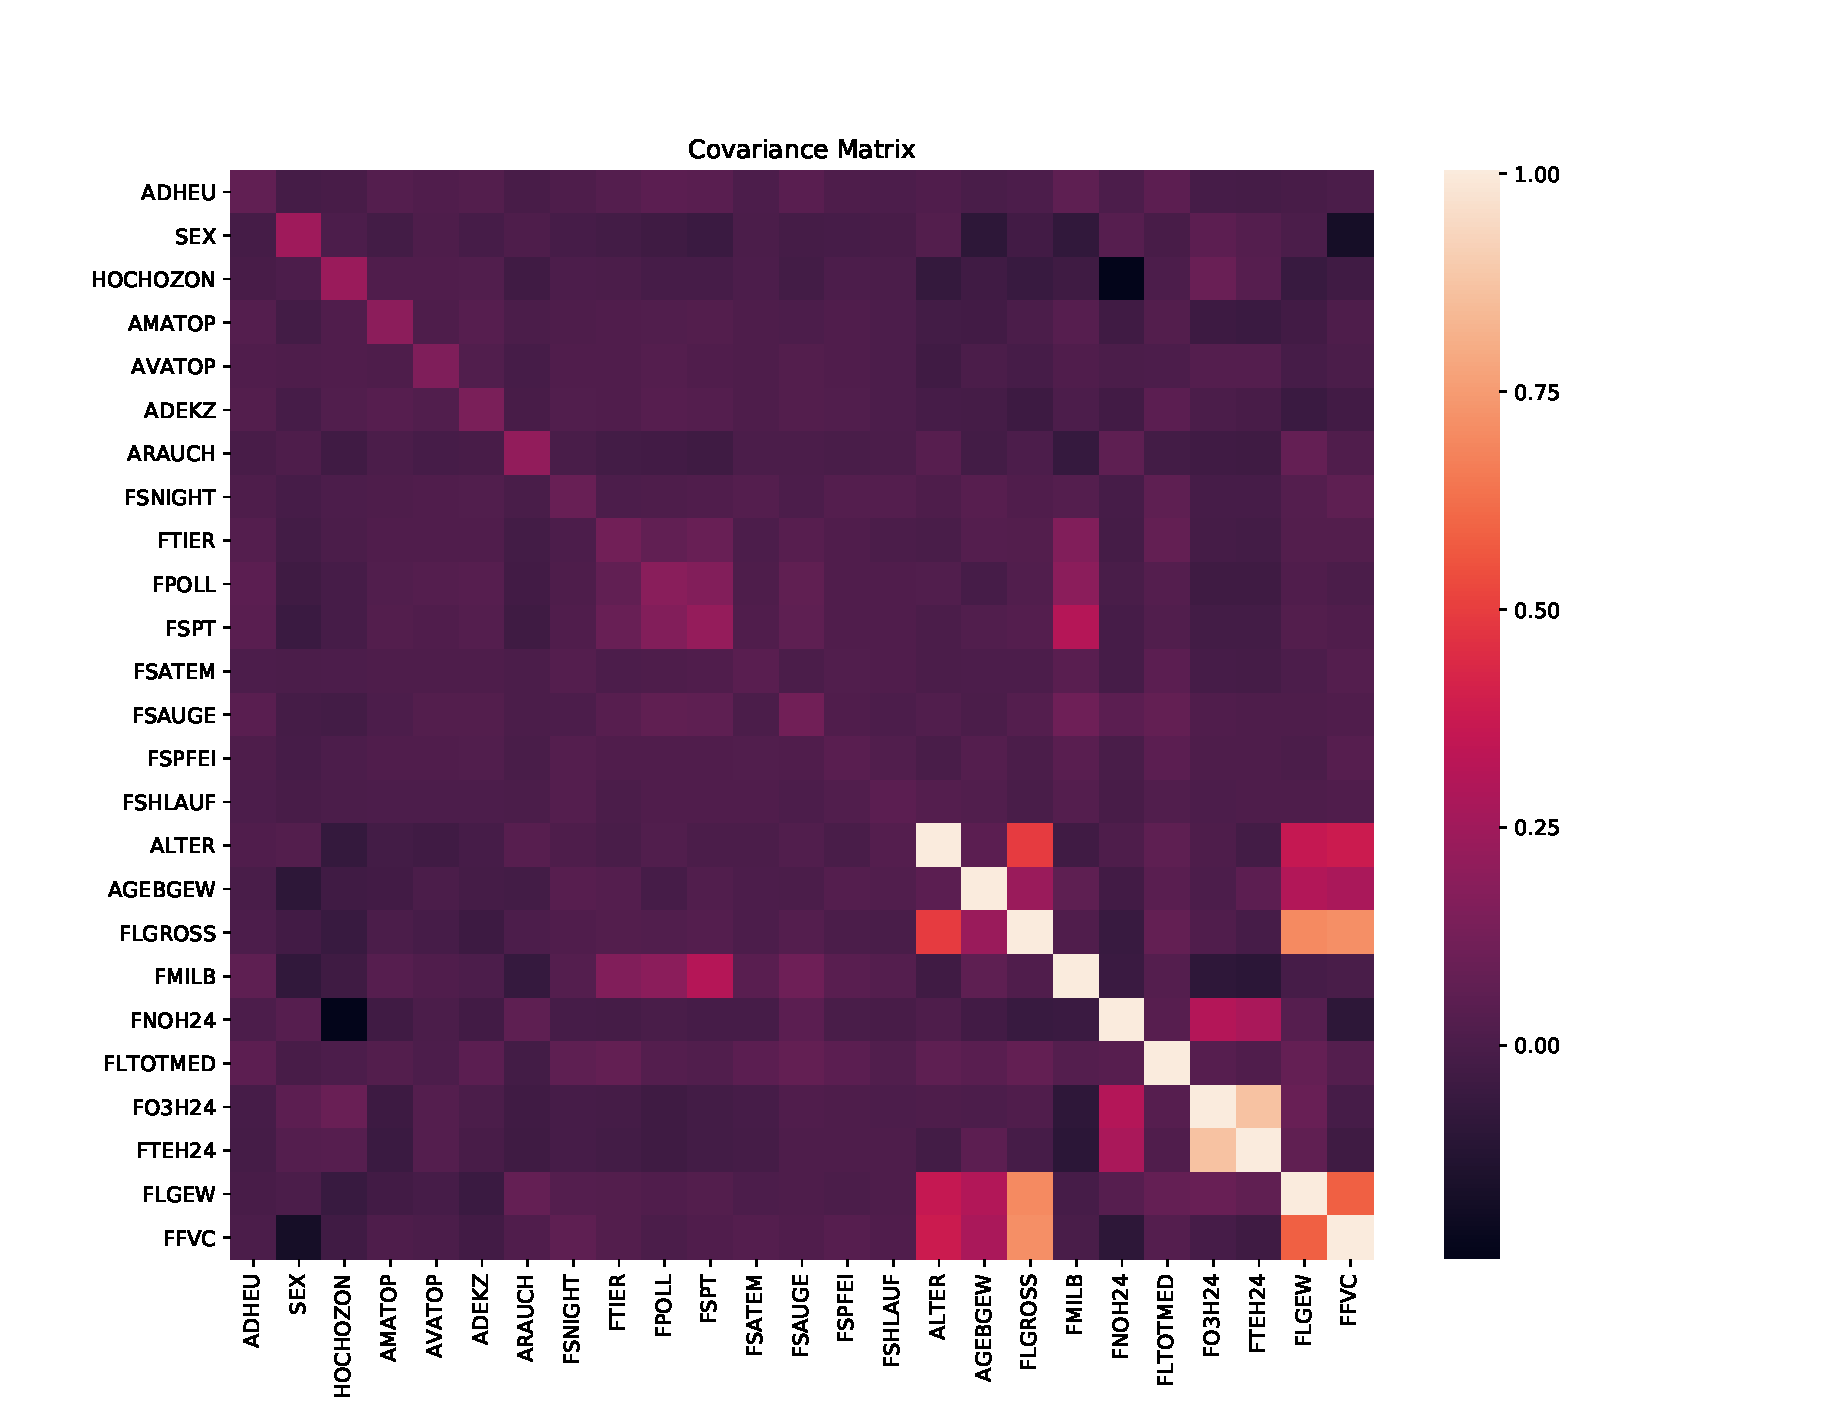
\includegraphics[width=0.8\textwidth]{figures/covheatmap.pdf}
	\caption{The covariance matrix of the data}
	\label{fig:covE1}
\end{figure}
Figure \ref{fig:cov_FFVC_E1} illustrates the covariance vector of the FFVC feature:
\begin{figure}[H]
	\centering
	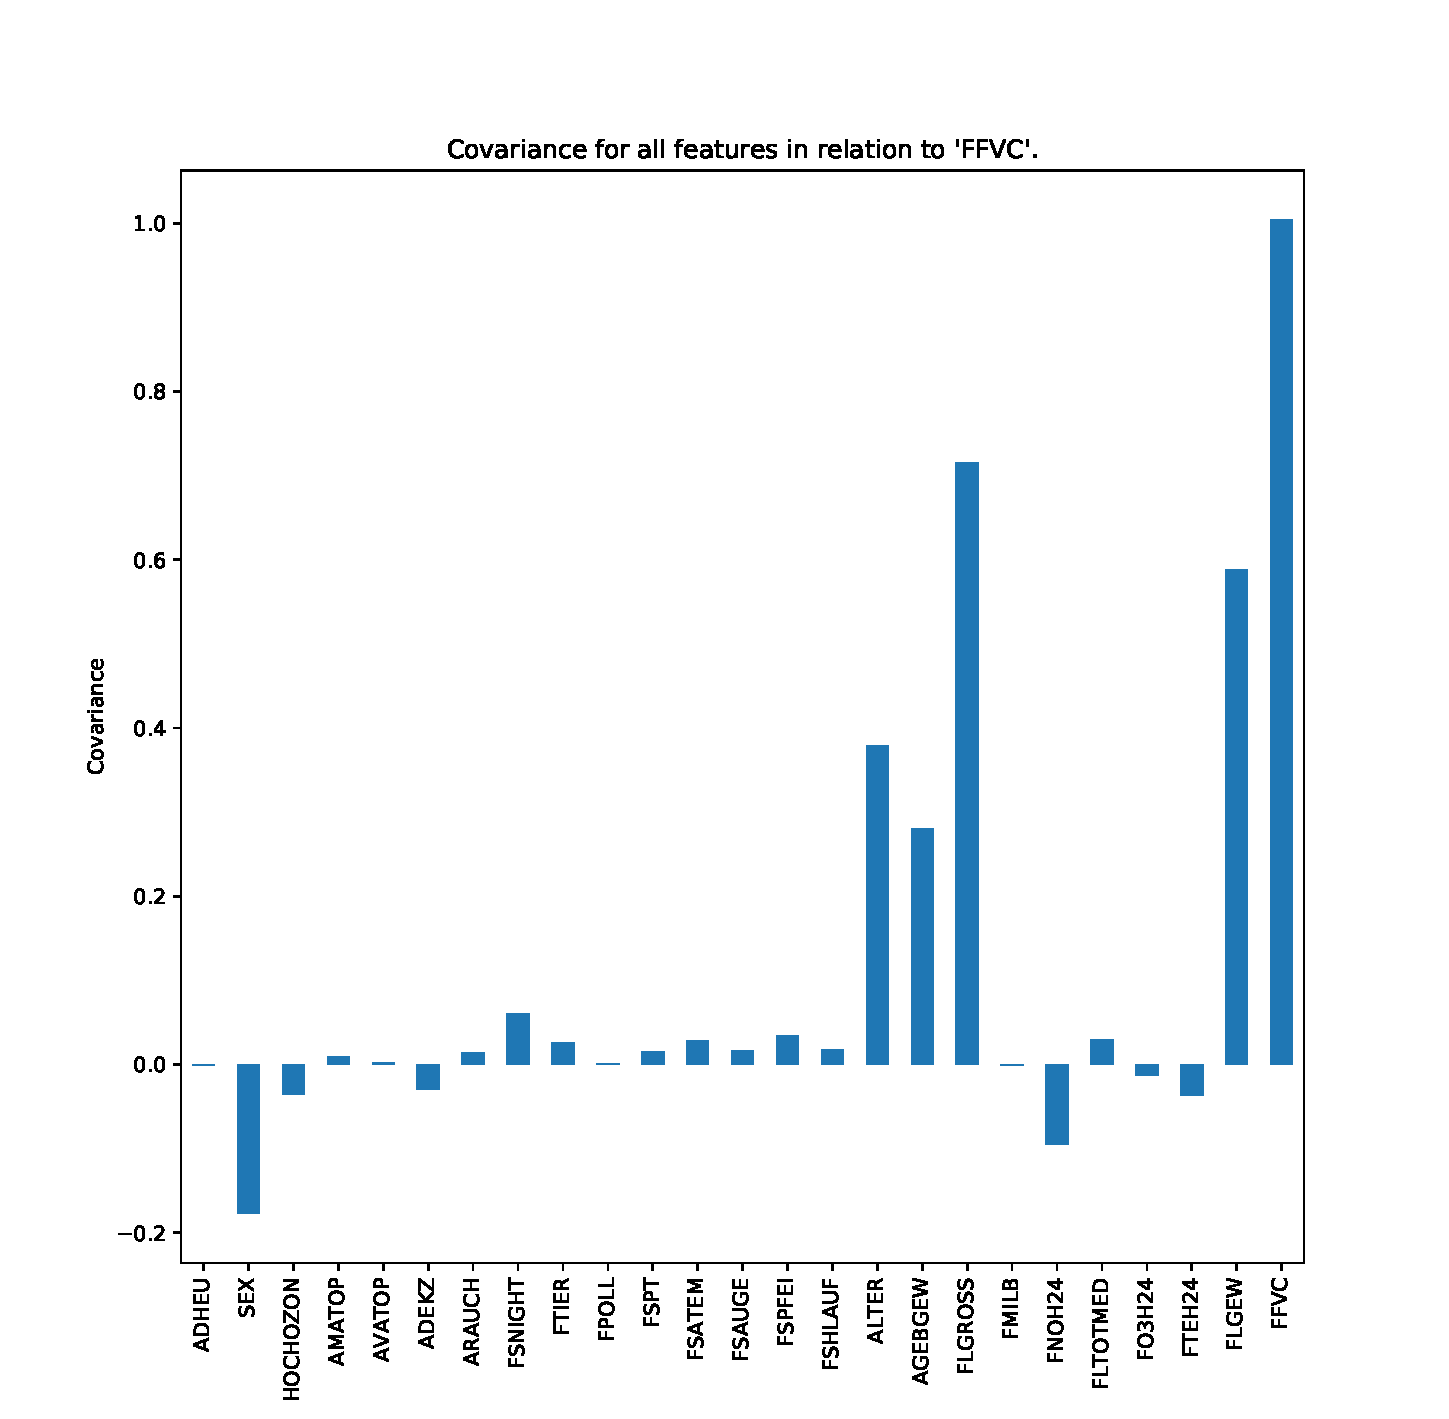
\includegraphics[width=0.8\textwidth]{figures/cov_FFVC_specific.pdf}
	\caption{The specific covariance of the FFVC features.}
	\label{fig:cov_FFVC_E1}
\end{figure}
%Figure \ref{fig:corrE1} illustrates the correlation matrix of the data:
%\begin{figure}[H]
%	\centering
%	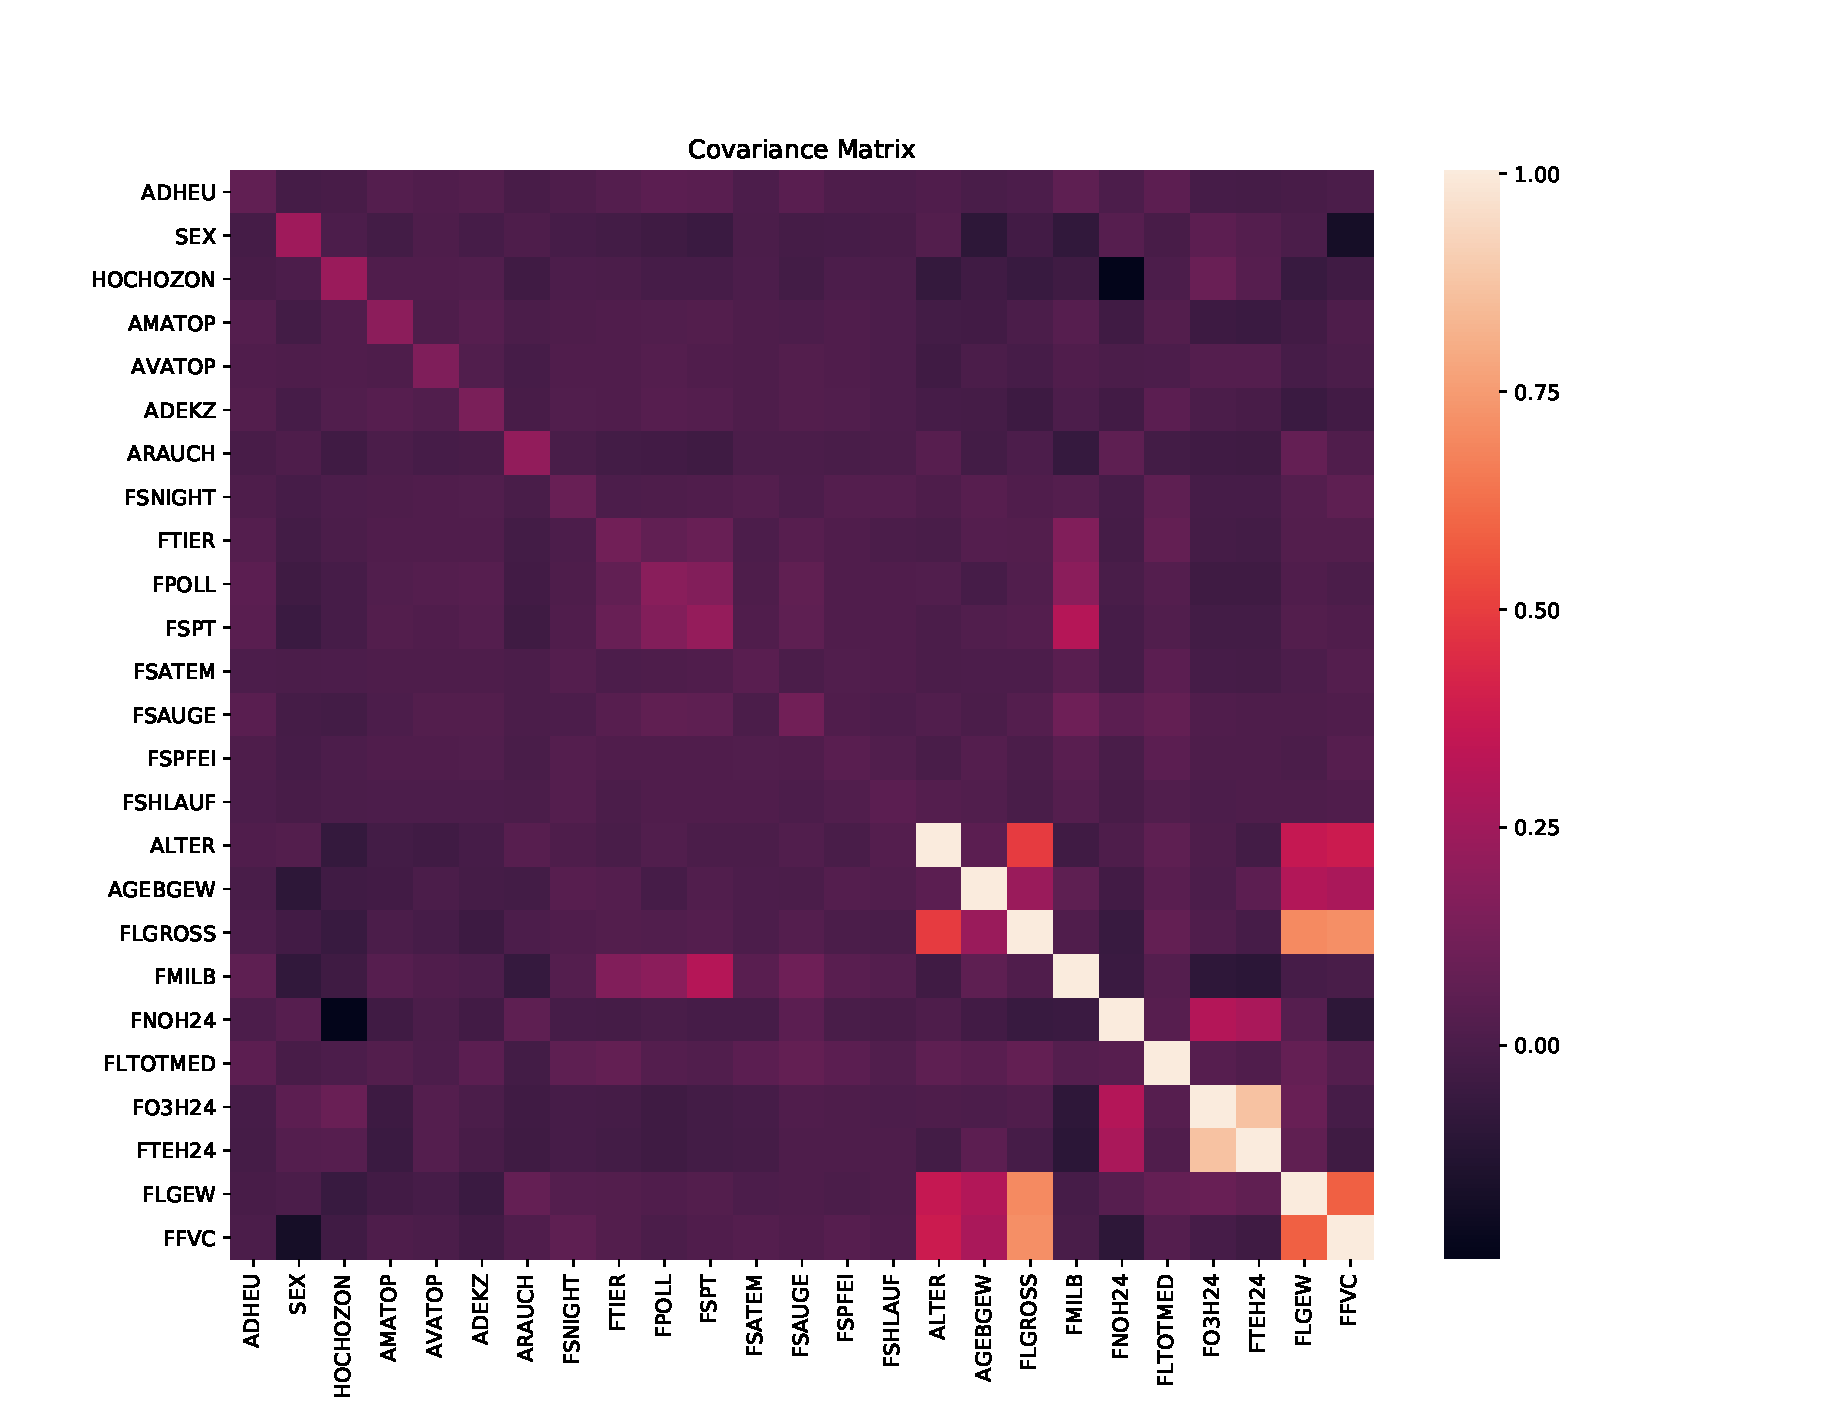
\includegraphics[width=0.8\textwidth]{figures/covheatmap.pdf}
%	\caption{The correlation matrix of the data}
%	\label{fig:corrE1}
%\end{figure}
%Figure \ref{fig:corr_FFVC_E1} illustrates the correlation vector of the FFVC feature:
%\begin{figure}[H]
%	\centering
%	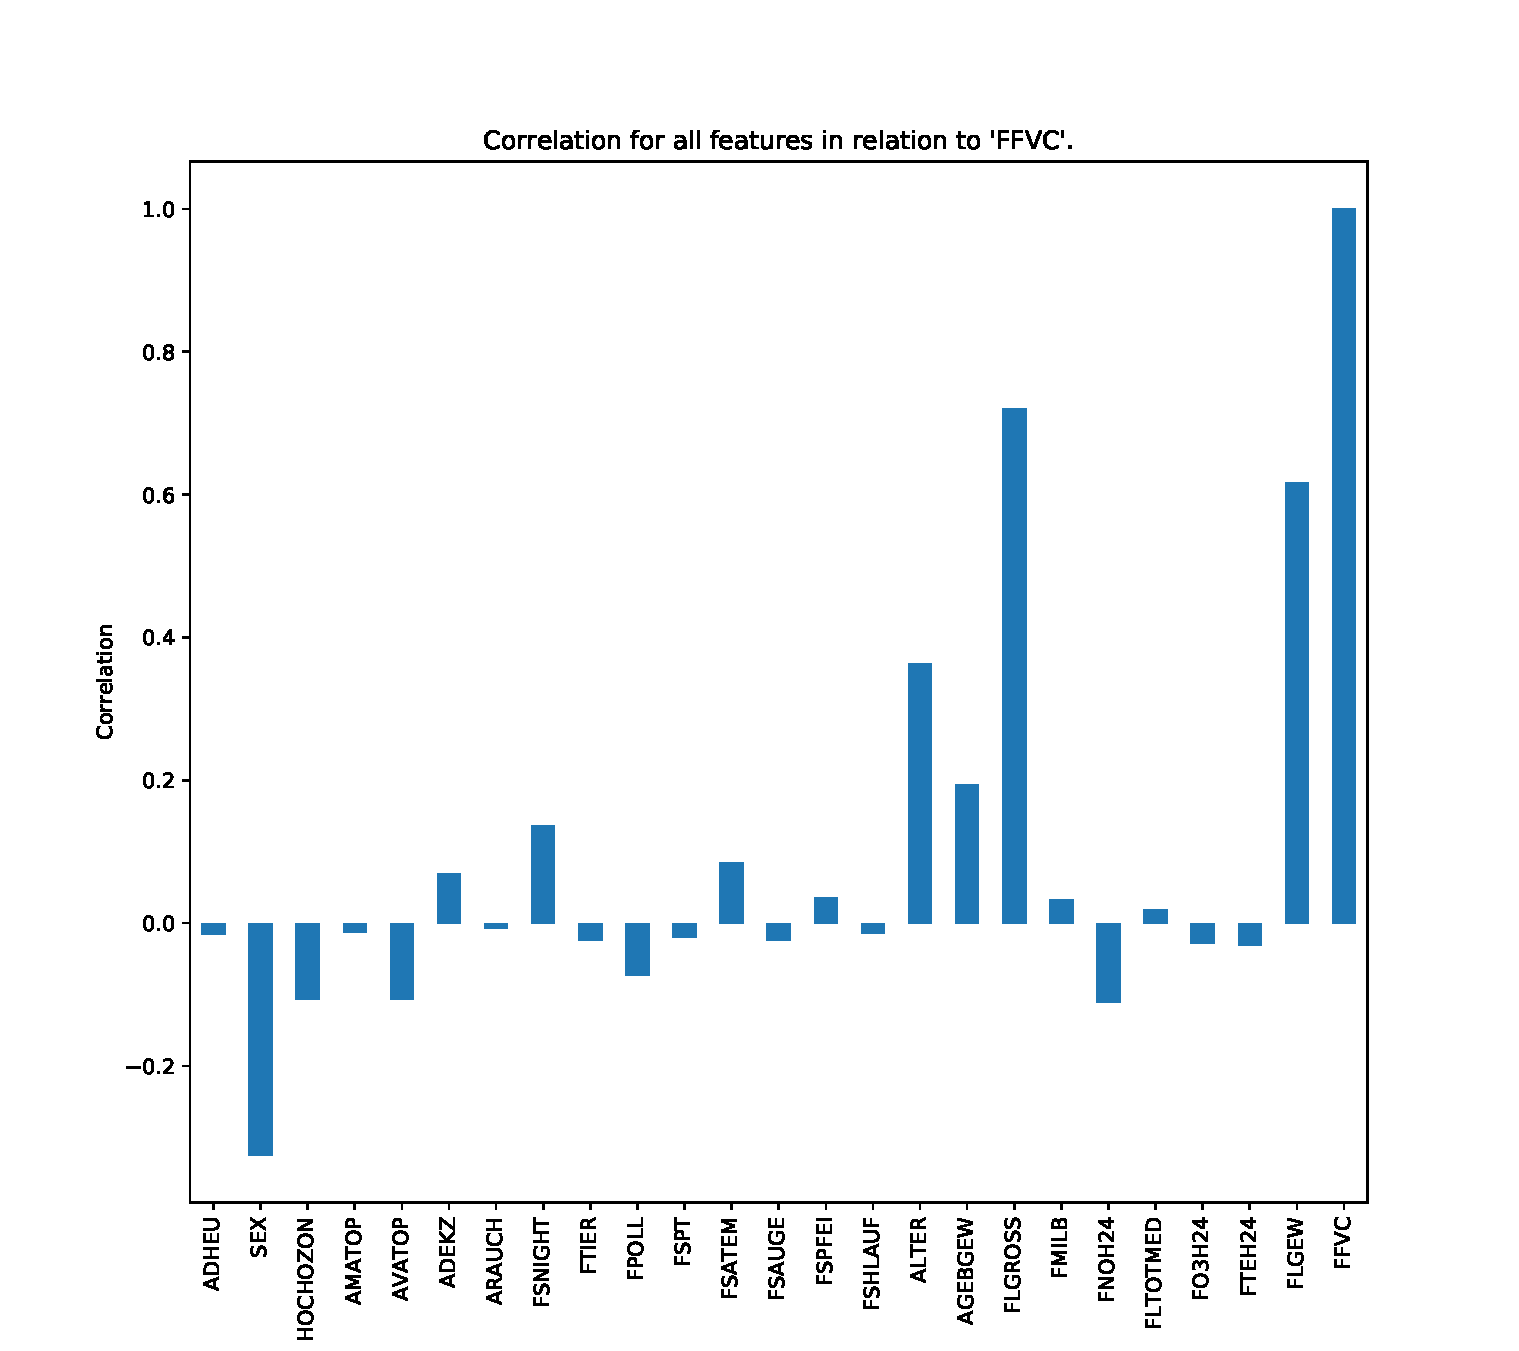
\includegraphics[width=0.8\textwidth]{figures/corr_FFVC_specific.pdf}
%	\caption{The specific correlation of the FFVC features.}
%	\label{fig:corr_FFVC_E1}
%\end{figure}
The covariate which has the strongest association with the forced vital capacity (FFVC) is the FLGROSS feature. Following is a report on the coefficient estimates, their standard error and the associated p-values:
\begin{figure}[H]
	\centering
	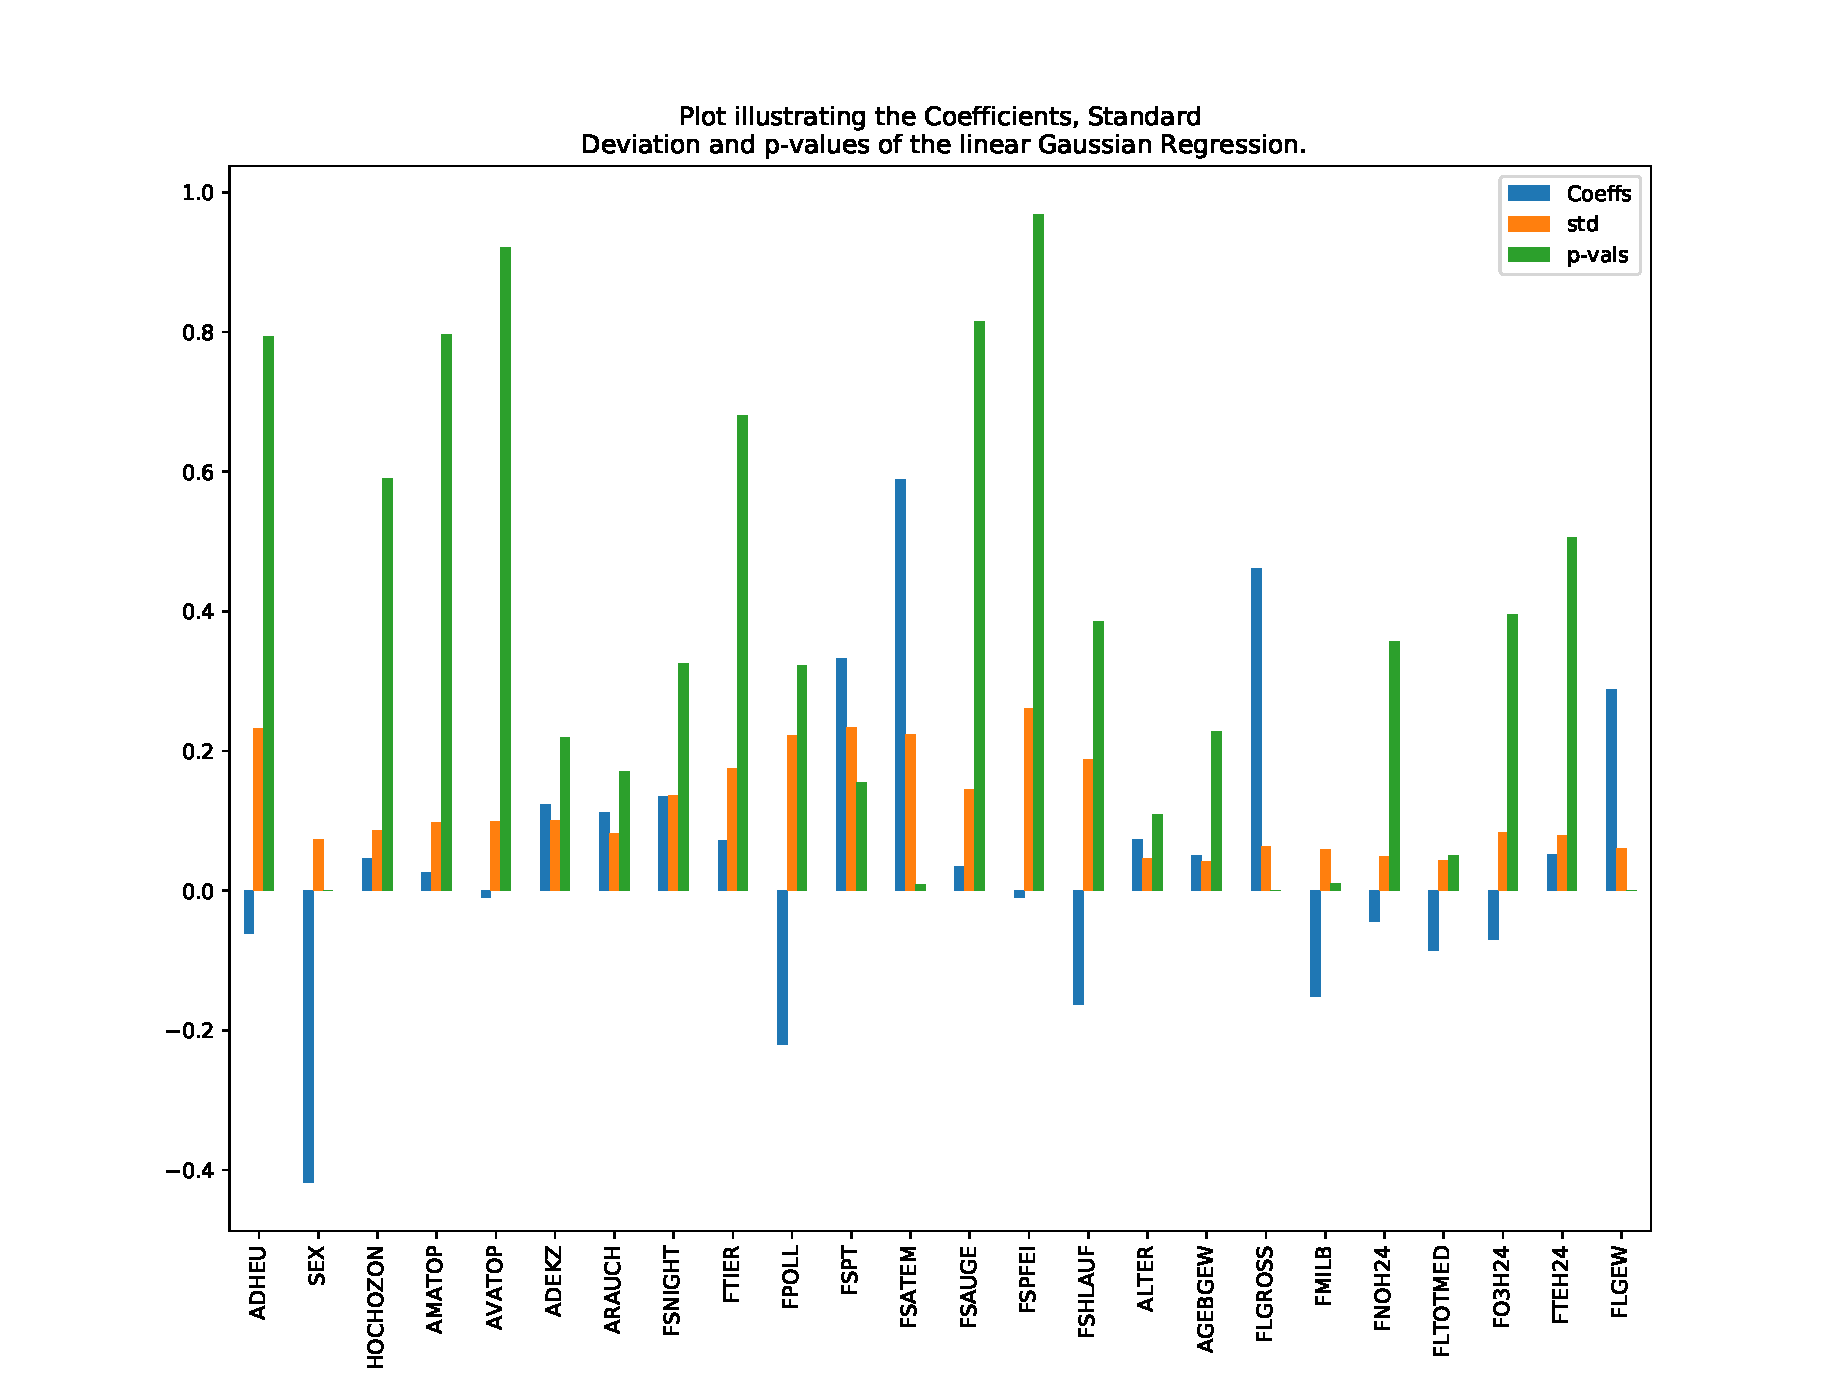
\includegraphics[width=0.8\textwidth]{figures/coefs_std_pvals.pdf}
	\caption{Figure illustrating the coefficients, standard deviations and p-values of all the features.}
	\label{fig:coefs_std_pval}
\end{figure}
It is clear that several of the p-values are quite large in relation to the typical p-value standard of $\sim 0.05$. It is also quite interesting to see in one figure the relation between the coefficient size and the p-value. It is clear to see for the 'SEX' and 'FSATEM' columns that the bigger the regression coefficient, the smaller the p-value of the feature. This can also be seen in the 'FLGROSS' column, which we remember from the covariance matrix as having the strongest association with the 'FFVC'. The opposite is also noticeable; the largest p-values, namely the 'FSPEI' and 'AVATOP' columns have coefficient values close to zero.\\\\ 
Some features do not exhibit this trend, such as the 'FSPT' and 'FPOLL' features exist somewhere in between, where they are not quite relevant to the prediction, but not quite irrelevant either.

\subsection*{3.}
The backwards and forwards selection algorithms performed using two different stopping criterion: One was 0.05 and the other was 0.1. Following are four figures of all these cases, where the coefficients, standard deviations, and all the p-values are listed in the same way as before.
\begin{figure}[H] 
	\label{ fig7} 
	\begin{minipage}[H]{0.5\linewidth}
		\centering
		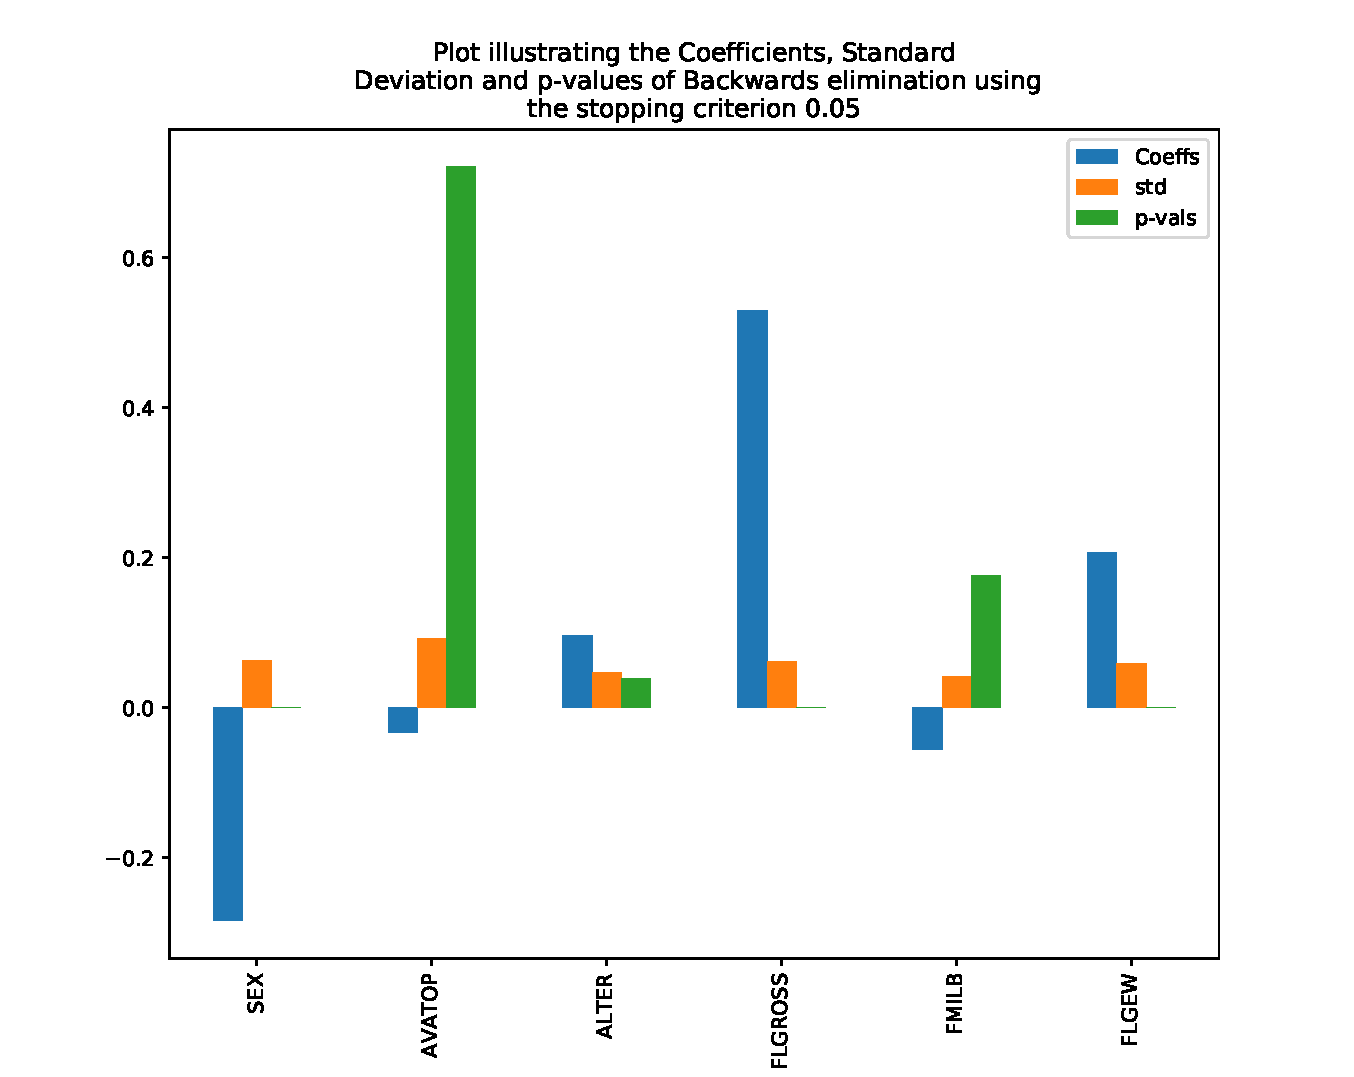
\includegraphics[width=1.11\linewidth]{figures/BS_005.pdf}
		\vspace{4ex}
	\end{minipage}%%
	\begin{minipage}[H]{0.5\linewidth}
		\centering
		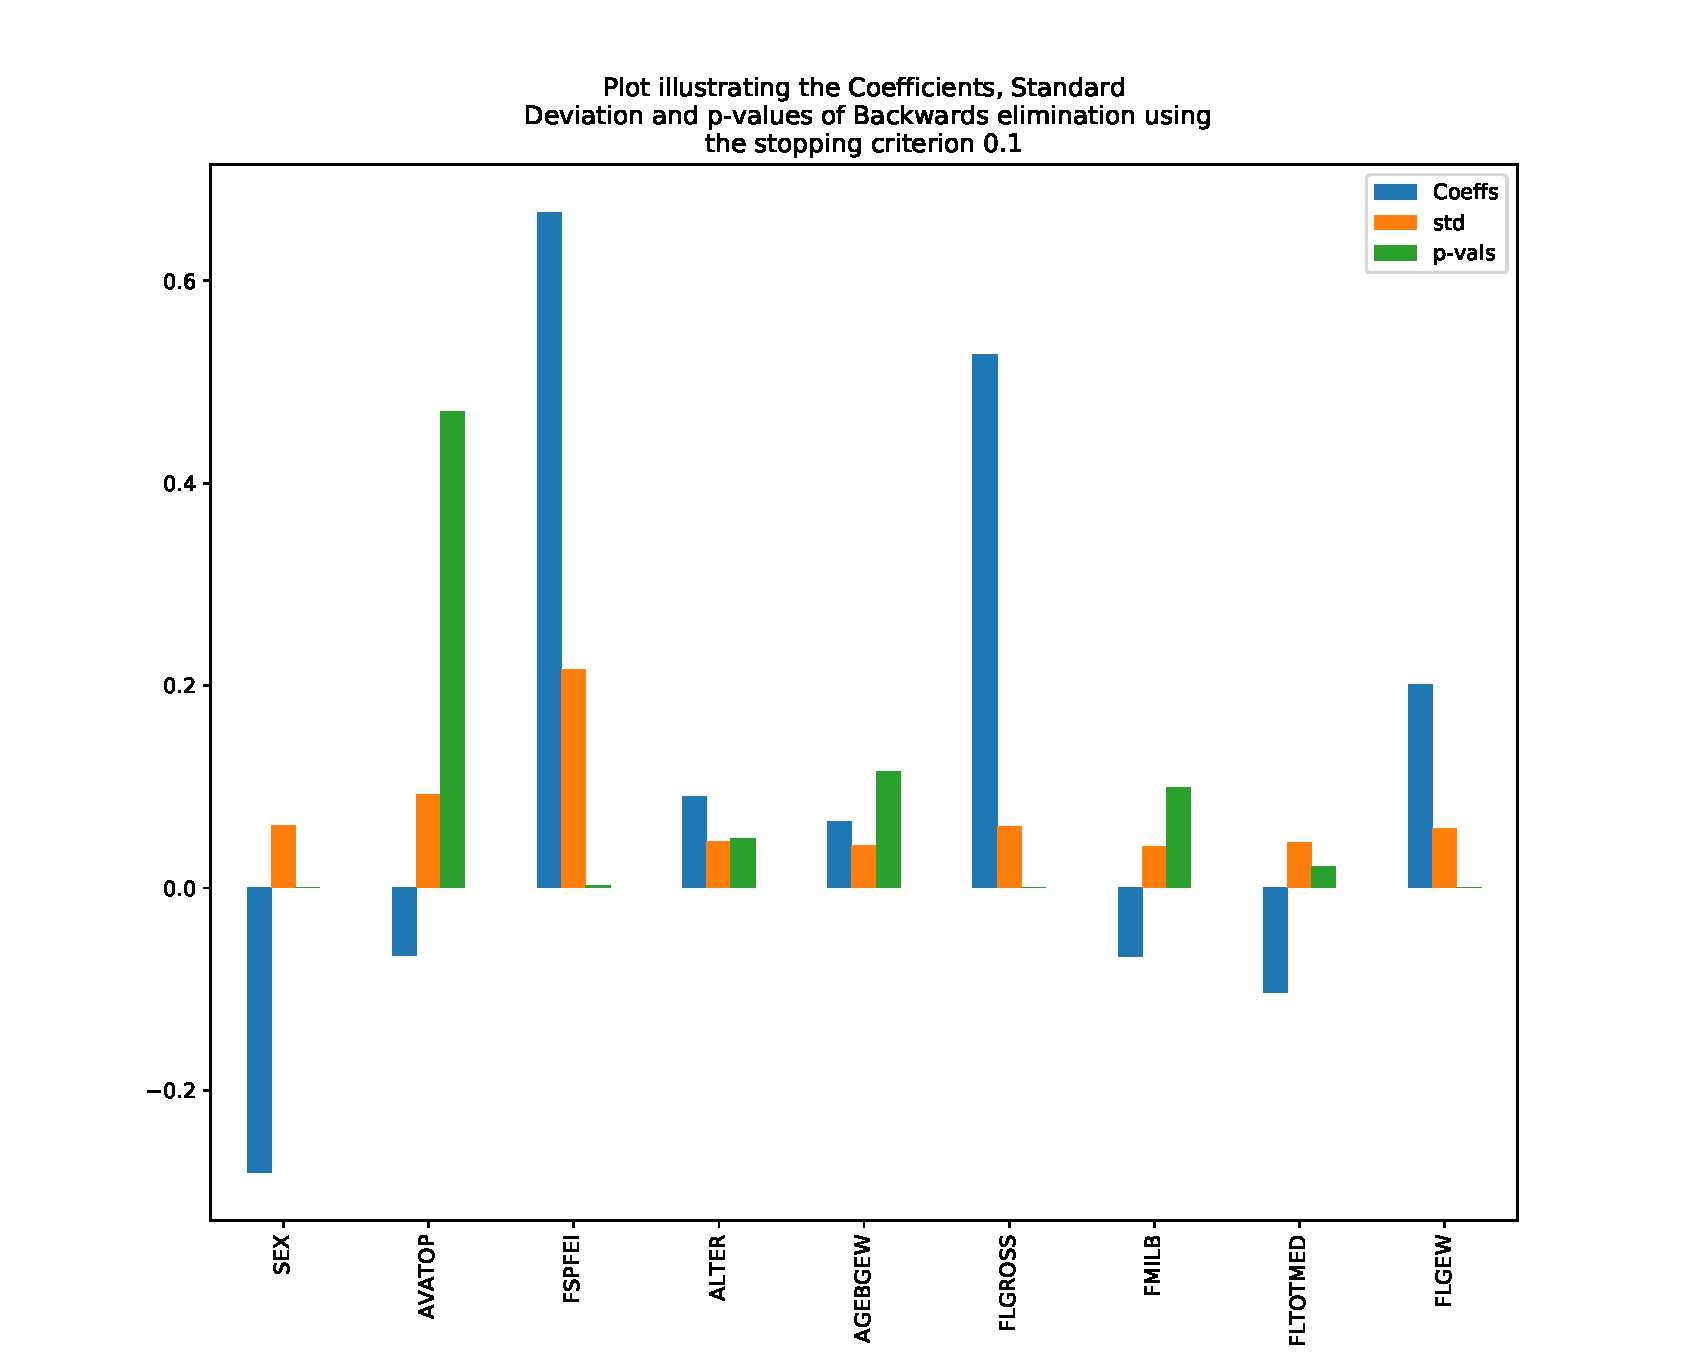
\includegraphics[width=1.11\linewidth]{figures/BS_01.pdf}
		\vspace{4ex}
	\end{minipage} 
	\begin{minipage}[H]{0.5\linewidth}
		\centering
		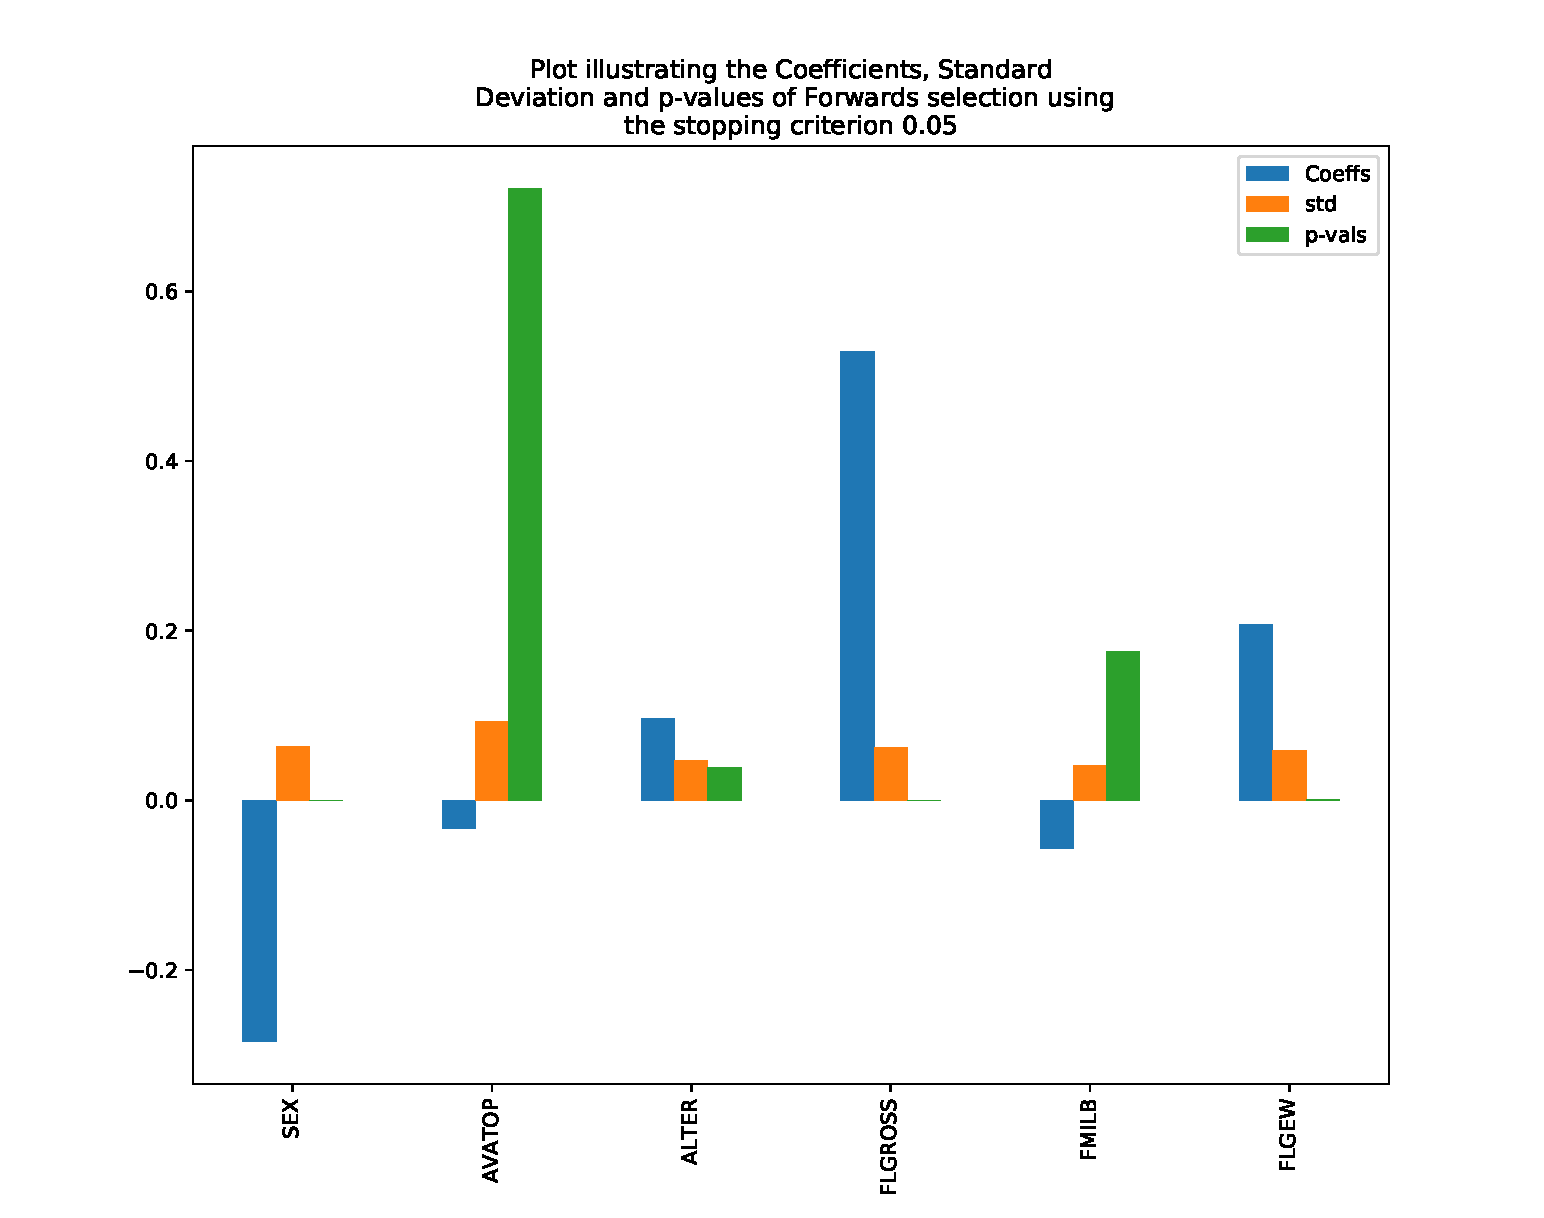
\includegraphics[width=1.11\linewidth]{figures/FS_005.pdf}
		\vspace{4ex}
	\end{minipage}%% 
	\begin{minipage}[H]{0.5\linewidth}
		\centering
		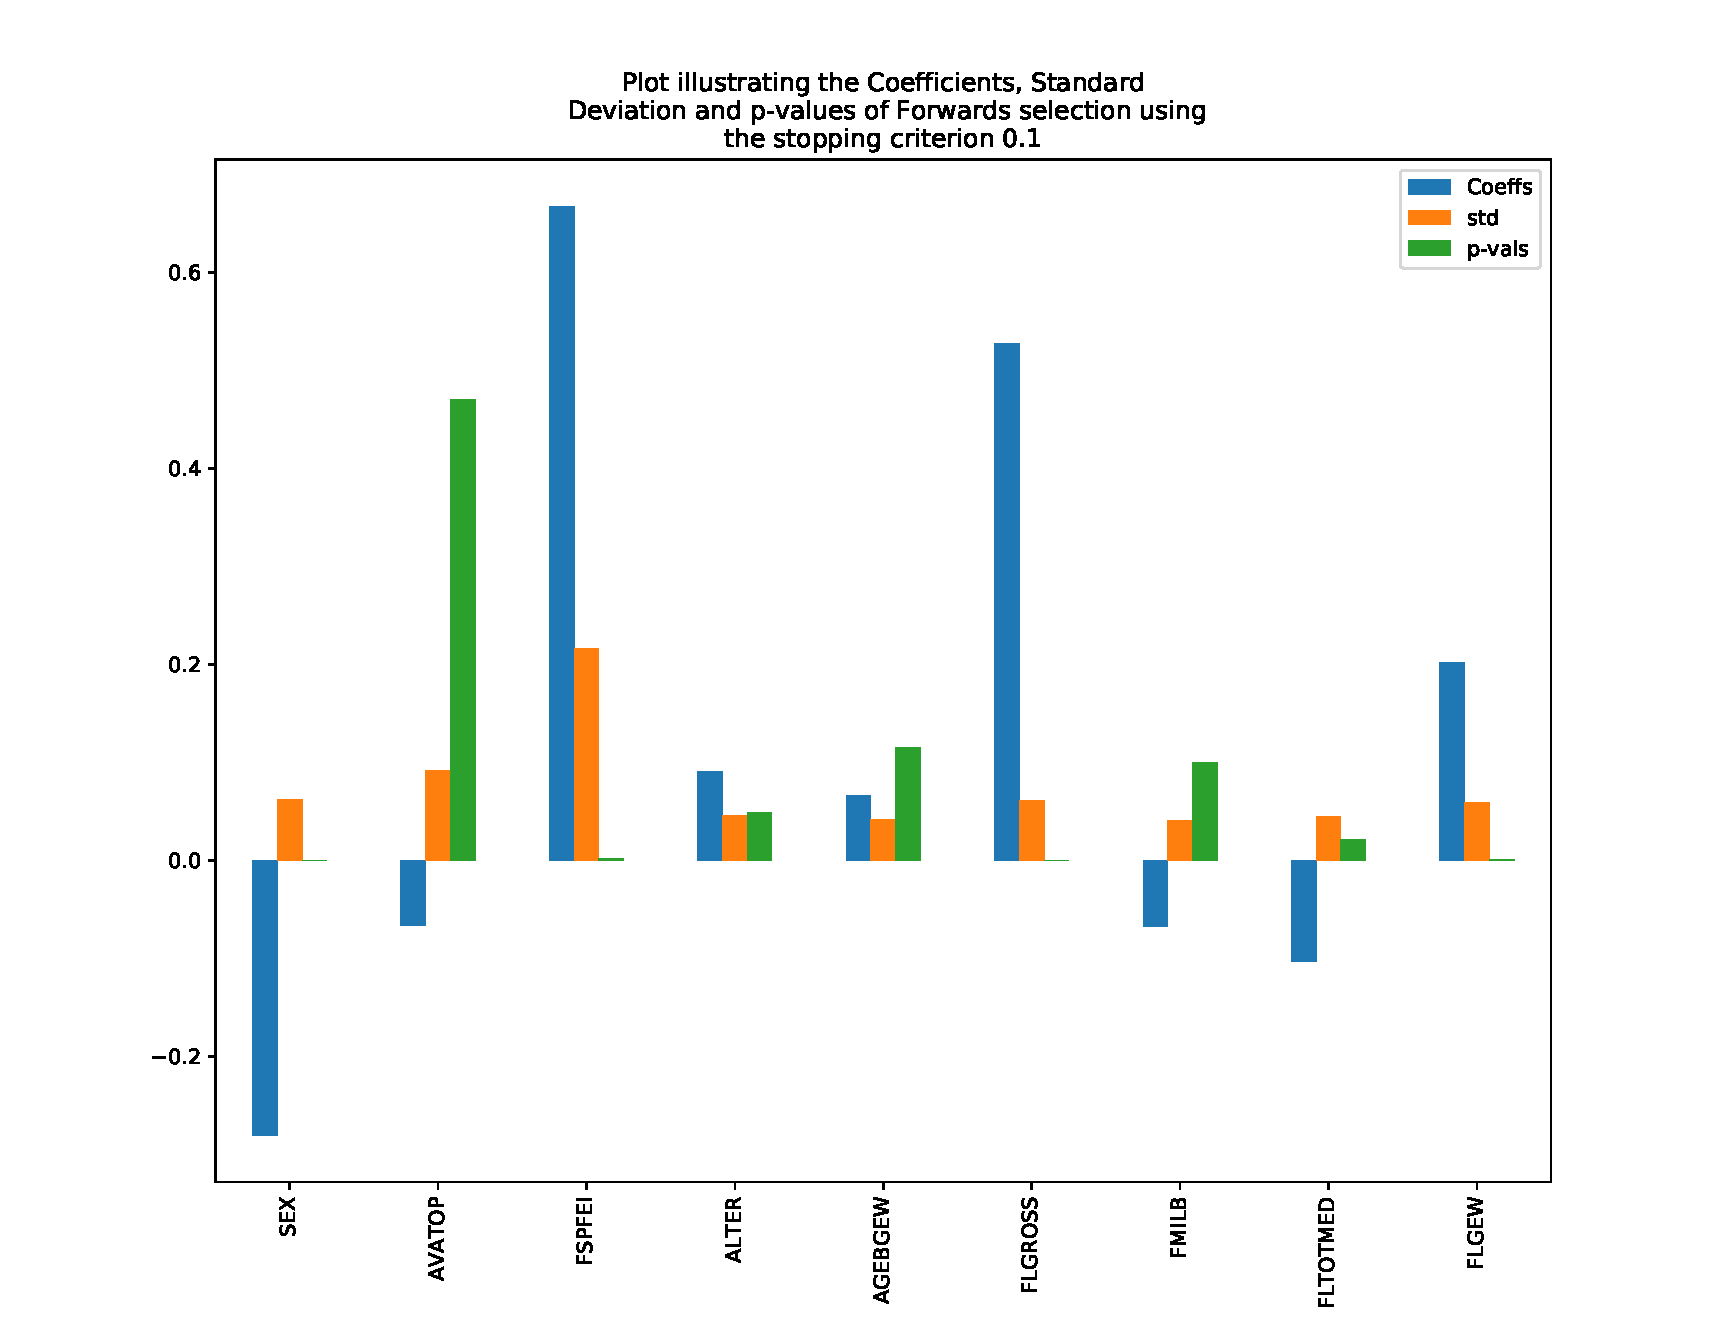
\includegraphics[width=1.11\linewidth]{figures/FS_01.pdf}
		\vspace{4ex}
	\end{minipage} 
\end{figure}
These are all quite similar predictions, as the backwards elimination and forwards selection essentially perform the same operation. They simply set a limit to the p-values, and filter out accordingly.\\\\
These methods are implemented in order to build a high quality regression model with little to no unnecessary features. This is done in a way that hopefully does not compromise the predictive abilities of the model, though some line must be drawn on this subject. Even features such as the 'FTIER' feature (see figure \ref{fig:coefs_std_pval}) helped in predicting the model somewhat. Although it was a feature that seemed to be quite linearly dependent, it still had some use. Removing this feature is not severely jeopardizing to the model's prediction, though some accuracy is lost. I therefore hypothesize that the mean-squared error will overall increase after the backwards elimination and forwards selection techniques.\\\\
Note, that when reproducing the following figures, there is a large amount of stochasticity in the data shuffling method. This means that the outcomes sometimes differ quite largely from one and other, so the figures illustrated in this report are simply one of many different cases.

\subsection*{4.}
Use both a bootstrap and k-fold CV method to find the best (in terms of deviance minimization) complexity parameter of a lasso regression.
Following is the bootstrap method results. The data was split up into 50/50, and the training data was further split up into $25\%$ testing data for the bootstrap samples. The $R^2$ scores were calculated using the average of a lot of bootstrap samples, for multiple hyperparameter $\alpha$ values. Figure \ref{fig:bootstrapE1} illustrates the results of this analysis:
\begin{figure}[H]
	\centering
	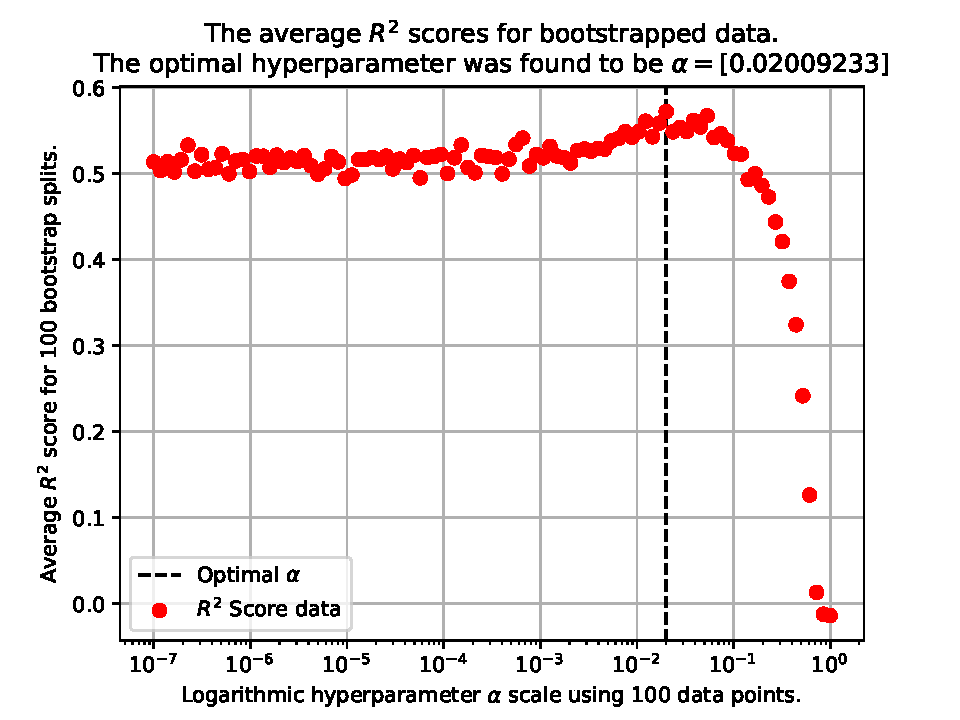
\includegraphics[width=0.8\textwidth]{figures/Bootstrap_E1.pdf}
	\caption{Figure illustrating the averages of the $R^2$ scores of multiple bootstrap samples. The optimal $\alpha$ parameter is found to be $\alpha=0.02$.}
	\label{fig:bootstrapE1}
\end{figure}

Doing the same for 5-fold CV, the two optimal $R^2$ scores are generated:

\begin{table}[H]
	\centering
	\caption{Maximum $R^2$ scores and minimum MSE scores of the two methods.}
	\begin{tabular}[t]{l@{\hskip 0.5in}c@{\hskip 0.5in}c}
		\toprule
		Scheme & Bootstrap & 5-fold CV \\
		\midrule
		 & & \\
		$R^2$ & 0.64222 & 0.56684 \\
		\bottomrule
	\end{tabular}
	\label{tab:E1P4}
\end{table}

\subsection*{5.}
Following are the results from the GAM simulations:

Only linear terms:
\begin{figure}[H]
	\centering
	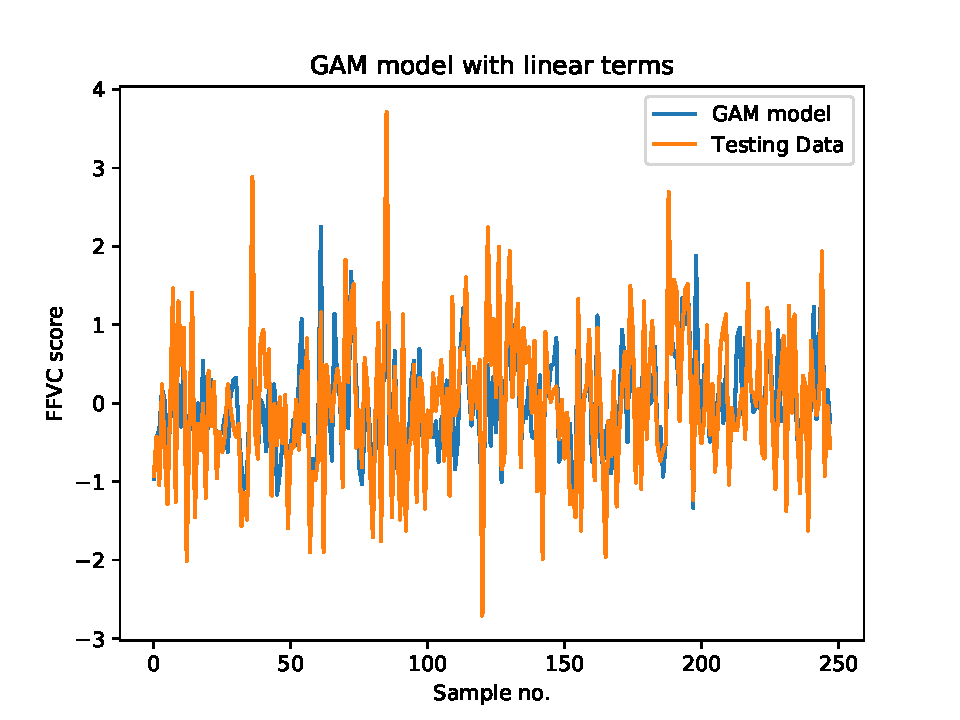
\includegraphics[width=0.8\textwidth]{figures/GAM1_E1.pdf}
	\caption{Figure illustrating the true FFVC scores vs the predicted scores using a GAM with only linear terms.}
	\label{fig:GAM1E1}
\end{figure}
Spline terms allowed:
\begin{figure}[H]
	\centering
	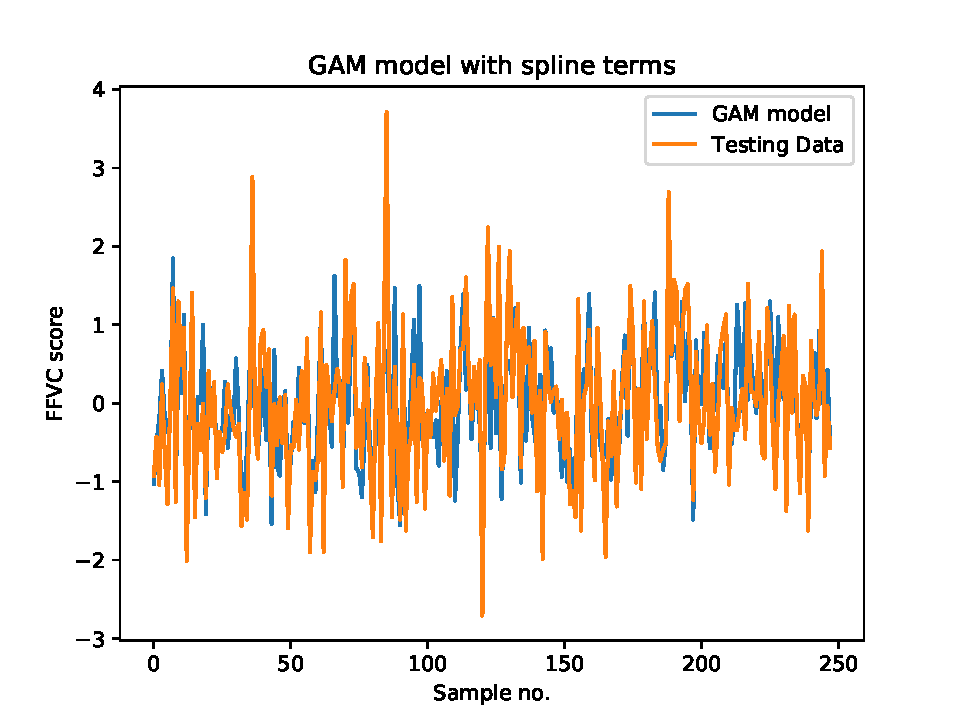
\includegraphics[width=0.8\textwidth]{figures/GAM2_E1.pdf}
	\caption{Figure illustrating the true FFVC scores vs the predicted scores using a GAM with splined, linear and polynomial terms.}
	\label{fig:GAM2E1}
\end{figure}
The 'only linear' GAM produced an MSE of 0.43756327\\

The 'splines and polynomial degrees allowed' GAM produced an MSE of 0.45348646.\\

These results are very chance-dependent, but in general the results are not too far off.

\subsection*{6.}
All the methods were successfully implemented using sklearns utilities. The results are illustrated in both the code and in the following section:

\subsection*{7.}
Following are the results of the code.


Linear Gauss of Exercise 1:
$$
MSE = 1.392
$$
Backwards- and Forwards models of Exercise 2:
MSE of Backwards Elimination 1 and 2:
$$
MSE1 = 1.377 
$$
and 
$$
MSE2 = 1.377
$$
MSE of Forwards Selection 1 and 2:
$$
MSE1 = 1.377
$$ 
and 
$$
MSE2 = 1.377
$$

Lasso results of Exercise 4:
Bootstrap achieved $R^2 = 0.617$
5-fold CV achieved $R^2 = 0.553$
GAM analysis from Exercise 5:
Linear only model $MSE = 0.343$
Polynomial allowed model $MSE = 0.441$
3 boosting models of Exercise 6:\\

i)   : MSE = 1.446\\

ii)  : MSE = 0.000\\

iii) : MSE = 1.378\\

The second result ii) is not correct, as the exercise was not properly accomplished. See the code for the attempt, however.

\section*{Exercise 2}
\subsection*{1.}
Figure \ref{fig:cumgains_kNN} illustrates the cumulative gains curve generated by the k-Nearest Neighbor method using $k=10$ and $33\%$ testing data.
\begin{figure}[H]
	\centering
	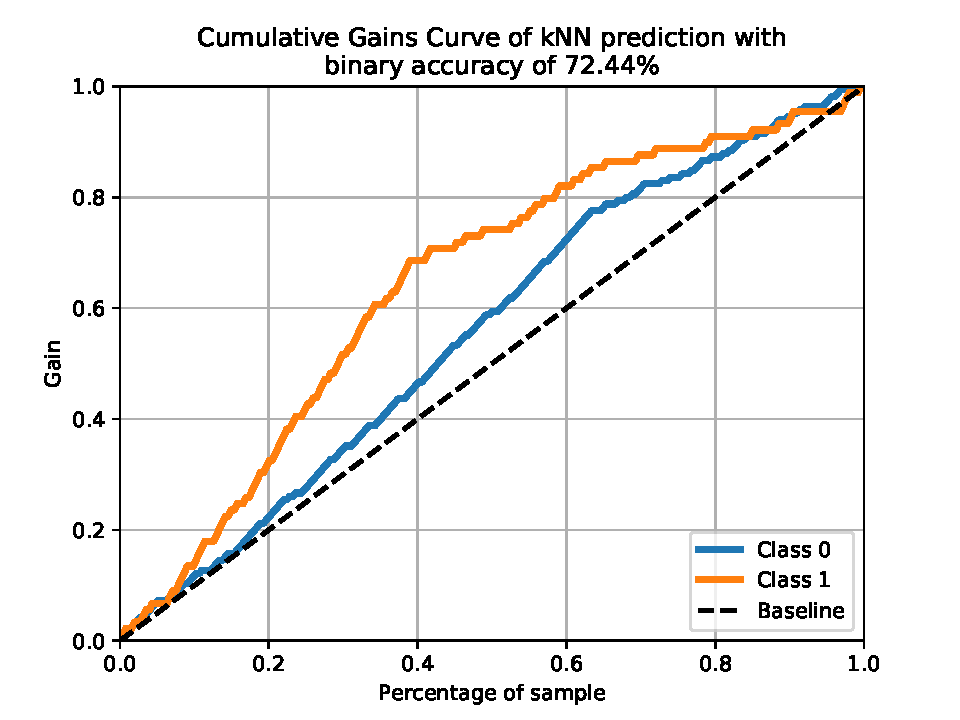
\includegraphics[width=0.8\textwidth]{figures/kNN_E2P1.pdf}
	\caption{Figure illustrating the averages of the $R^2$ scores of multiple bootstrap samples. The optimal $\alpha$ parameter is found to be $\alpha=0.02$.}
	\label{fig:cumgains_kNN}
\end{figure}
Figure \ref{fig:kNN_k} illustrates an analysis of which k value produces the optimal score:
\begin{figure}[H]
	\centering
	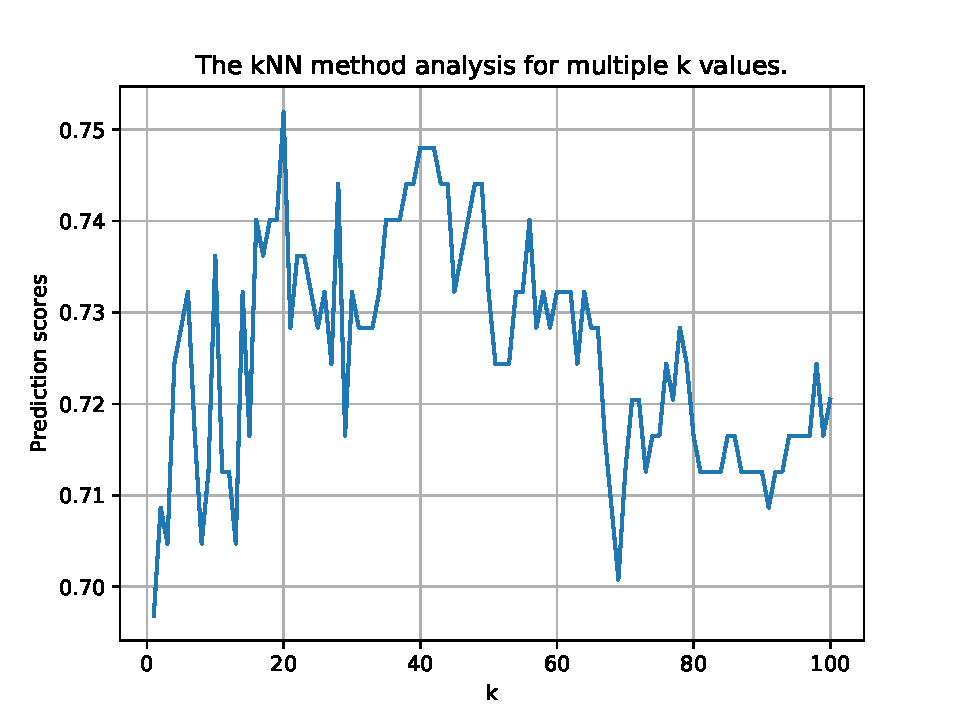
\includegraphics[width=0.8\textwidth]{figures/E1P2_kNN.pdf}
	\caption{Figure illustrating the averages of the $R^2$ scores of multiple $k$ values.}
	\label{fig:kNN_k}
\end{figure}

\subsection*{2.}
Figure \ref{fig:GAMRES} illustrates the prediction results for the GAM method using splines only. 
\begin{figure}[H]
	\centering
	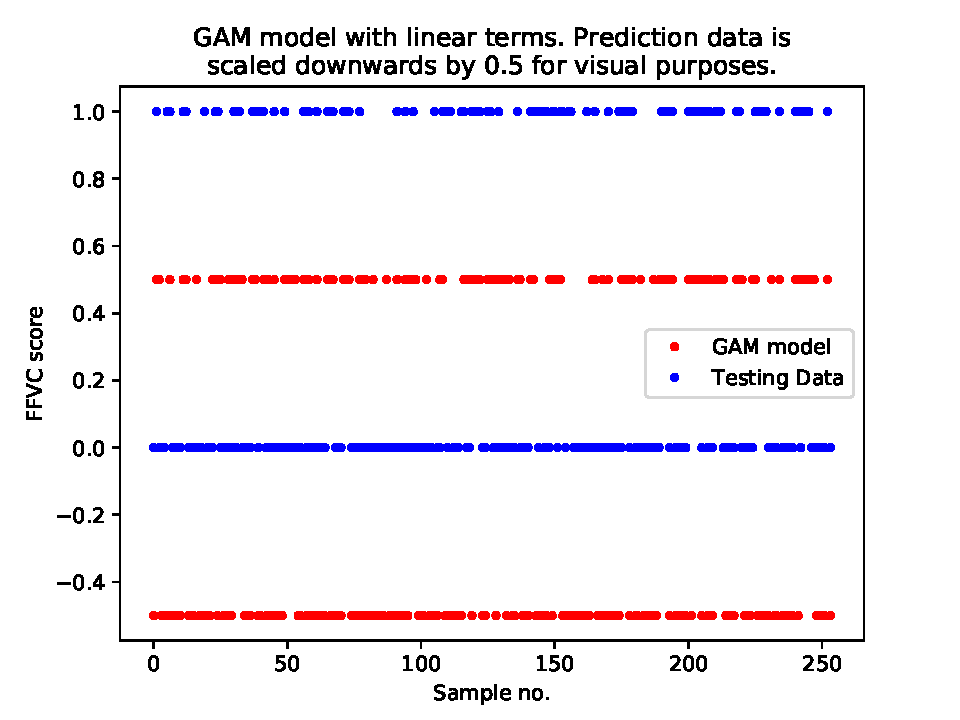
\includegraphics[width=0.8\textwidth]{figures/GAM_RESULTS.pdf}
	\caption{GAM results for exercise 2.}
	\label{fig:GAMRES}
\end{figure}

\subsection*{3.}
This was implemented into the python program using sklearn's functionalities. Bagging with both voting and averaging was unfortunately not accomplished, however.

\subsection*{4.}
Table \ref{tab:ALMOST} illustrates the results of all these methods.
\begin{table}[H]
	\centering
	\caption{Scores for all the methods from exercise 3.}
	\begin{tabular}[t]{l@{\hskip 0.5in}c}
		\toprule
		Scheme & Score \\
		\midrule
		Decision Tree score:&	 0.6654\\
		Bagging score:  	 &0.7244\\
		Random Forest score:&	 0.7244\\
		Neural Network score:&	 0.7047\\
		ADA Boost score:	 &0.7047\\
		\bottomrule
	\end{tabular}
	\label{tab:ALMOST}
\end{table}


If I were to choose between these models, I would choose the bagging or the random forest method. This choice is due to the score performances. However, all these methods are very reliable, and upon multiple runs of the code, they are all found to have large deviations (oscillations) depending on the randomness seed. This would be interesting to study further.


\subsection*{5.}
Following are the new figures, just with the outliers removed. The figures illustrate the same phenomenon as before:
\begin{figure}[H]
	\centering
	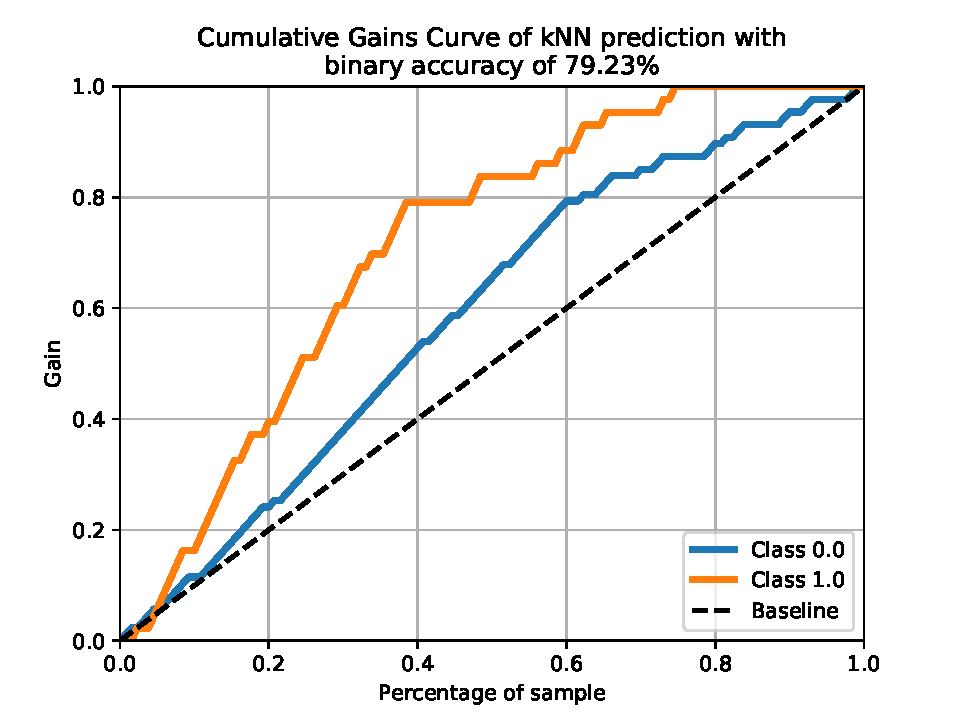
\includegraphics[width=0.8\textwidth]{figures/LASTONE.pdf}
	\label{fig:LASTONE}
\end{figure}
\begin{figure}[H]
	\centering
	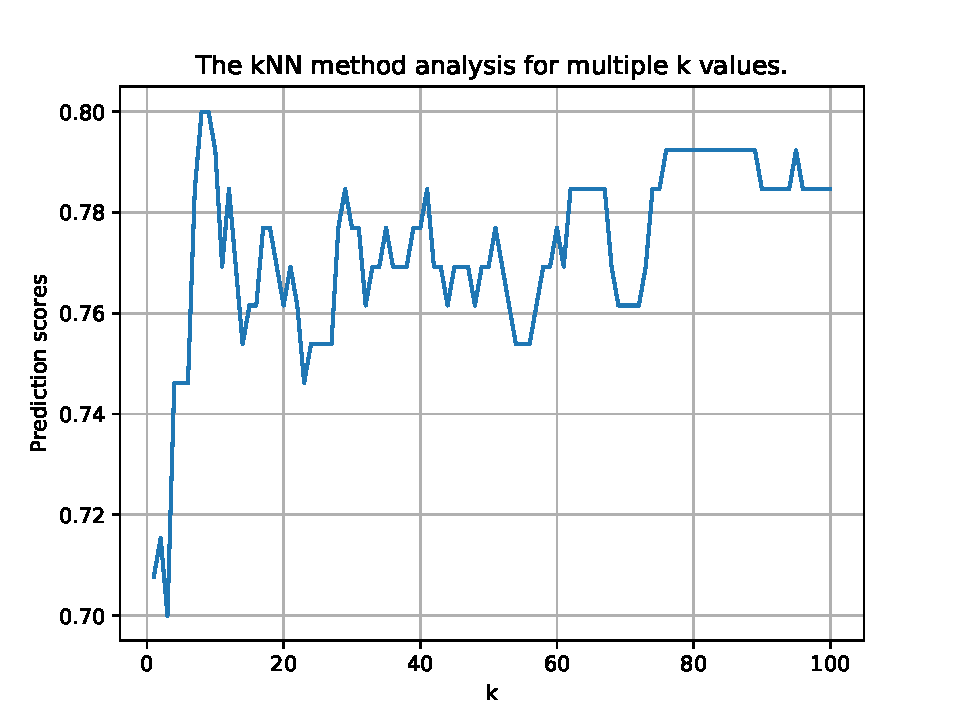
\includegraphics[width=0.8\textwidth]{figures/LASTTWO.pdf}
	\label{fig:LASTTWO}
\end{figure}
\begin{figure}[H]
	\centering
	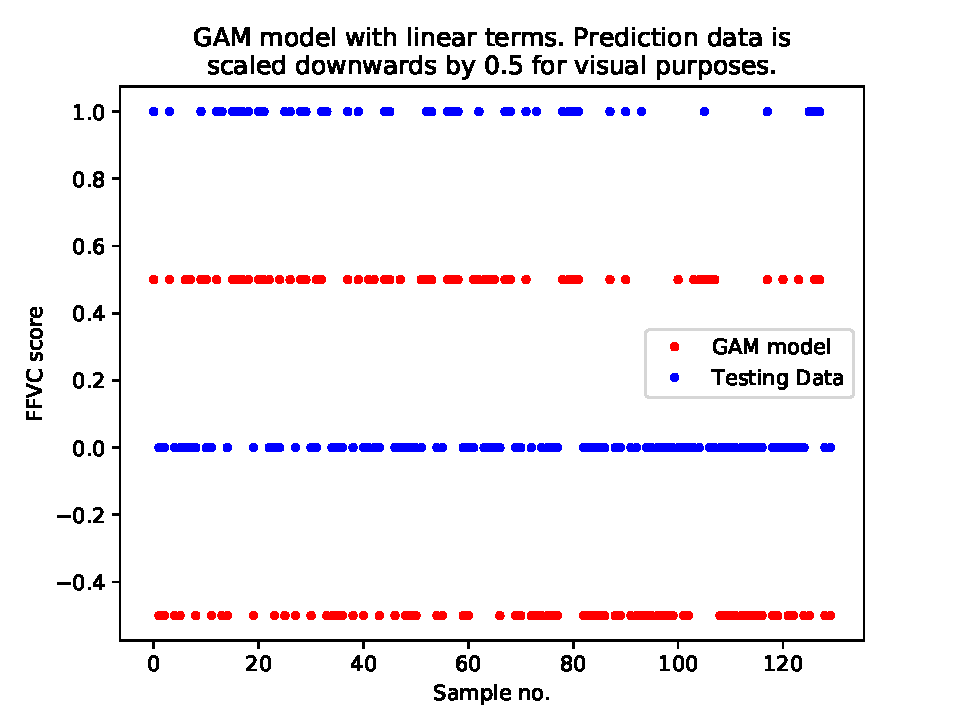
\includegraphics[width=0.8\textwidth]{figures/LASTTHREE.pdf}
	\label{fig:LASTTHREE}
\end{figure}

Following are the results again:

\begin{table}[H]
	\centering
	\caption{Scores for all the methods with outliers removed.}
	\begin{tabular}[t]{l@{\hskip 0.5in}c}
		\toprule
		Scheme & Score \\
		\midrule
		Decision Tree score:&	 0.6692\\
		Bagging score:  	& 0.7385\\
		Random Forest score:&	 0.7923\\
		Neural Network score:&	 0.7462\\
		ADA Boost score:	 &0.7385\\
		\bottomrule
	\end{tabular}
	\label{tab:LASTONE}
\end{table}




% References
\section*{References}
McLeod, S. A. (2019, May 20). What a p-value Tells You About Statistical significance. Simply Psychology. https://www.simplypsychology.org/p-value.html


\section*{Code}
The code is as follows (the project folder can be found on my github, as described previously):
\subsection*{main.py}
\begin{lstlisting}[language=Python]
import numpy as np
import pandas as pd
import matplotlib.pyplot as plt
import sklearn
import sklearn.model_selection
import sklearn.preprocessing
from lib.Ex1 import Exercise1
from lib.Ex2 import Exercise2

"""
Project 2 for STK-IN4300 Folder.
--------------------------------
Recommend running the code using:

```
$ python3 main.py -W ignore
```

This helps with the error messages
produced by several of the modules.
The modules used in solving this
project include numpy, sklearn,
seaborn, imblearn, pandas and many
more.
"""


def main():
	Task1()   # Done.
	# Task2()     # Done. Bagging with probabilities was not accomplished.
	return 0

def Task1():
	e1 = Exercise1()
	e1.plot = False     # whether to see the plots or not. There are many.
	print("==============")
	print("Exercise 1.1:")
	print("==============")
	e1.scale_data()             # Exercise 1.   Done.
	print("==============")
	print("Exercise 1.2:")
	print("==============")
	e1.linear_Gauss()           # Exercise 2.   Done.
	print("==============")
	print("Exercise 1.3:")
	print("==============")
	e1.bf_selection1()          # Exercise 3.   Done.
	print("==============")
	print("Exercise 1.4:")
	print("==============")
	e1.boot_CV_compare()        # Exercise 4.   Done.
	print("==============")
	print("Exercise 1.5:")'.source.python:not(.string)':
	'self':
	'prefix': '.'
	disabled: true
	print("==============")
	e1.GAM1()                   # Exercise 5.   Done.
	print("==============")
	print("Exercise 1.6:")
	print("==============")
	e1.comp_boosting()          # Exercise 6.   Done. Could not Spline Boost.
	print("==============")
	print("Exercise 1.7:")
	print("==============")
	e1.report_points()          # Exercise 7.   Done.
	print("==============")
	print("Problem 1 Complete.")
	print("==============")

def Task2():
	e2 = Exercise2()
	e2.plot = False     # whether to see plots.
	e2.process_data()           # Necessary for Exercises 1, 2, 3, and 4
	print("==============")
	print("Exercise 2.1:")
	print("==============")
	e2.k_NN()                   # Exercise 1.   Done
	print("==============")
	print("Exercise 2.2:")
	print("==============")
	e2.GAM2()                   # Exercise 2.   Done.
	print("==============")
	print("Exercise 2.3:")
	print("==============")
	e2.tree_bag_ada()           # Exercise 3.   Done.
	print("==============")
	print("Exercise 2.4:")
	print("==============")
	e2.best_method()            # Exercise 4.   Done.
	print("==============")
	print("Exercise 2.5:")
	print("==============")
	e2.remove_outliers()        # Exercise 5.   Done.
	print("==============")
	print("Problem 2 Complete.")
	print("==============")

if __name__ == '__main__':
	main()

\end{lstlisting}
Following then is the code written for exercise 1:
\subsection*{lib/Ex1.py}
\begin{lstlisting}[language=Python]
import pandas as pd
import numpy as np
import sklearn
import matplotlib.pyplot as plt
import seaborn as sb
import sklearn.model_selection
import sklearn.preprocessing
# from sklearn import cross_validation
from sklearn.model_selection import cross_validate
from sklearn.model_selection import ShuffleSplit
from sklearn.linear_model import LassoCV
from sklearn import linear_model
import statsmodels.api as sm


class Exercise1:
	def __init__(self):
		pass

	def scale_data(self):
		"""Analysis of the 496 children with 24 features. Takes in argument 'sc'
		which indicates how the data should be split into training/testing data.
		So far takes in arguments sc='50/50' for 50% splitting, sc='index', for
		custom indices to be used for splitting (used in bootstrap and k-fold
		cross validation methods)."""
		df = pd.read_csv('ozone_data.txt', sep = ' ')
		"""
		'Column nr.'    'Column name'
		Columns to scale:
		1   ALTER
		9   AGEBGEW
		11  FLGROSS
		12  FMILB
		13  FNOH24
		16  FLTOTMED
		17  FO3H24
		19  FTEH24
		22  FLGEW
		25  FFVC
		One-Hot columns:
		2   ADHEU;
		3   SEX;
		4   HOCHOZON;
		5   AMATOP;
		6   AVATOP;
		7   ADEKZ;
		8   ARAUCH
		10  FSNIGHT
		14  FTIER
		15  FPOLL
		18  FSPT
		20  FSATEM
		21  FSAUGE
		23  FSPFEI
		24  FSHLAUF
		"""
		scale_inds = [0, 8, 10, 11, 12, 15, 16, 18, 21, 24]
		oneht_inds = [1, 2, 3, 4, 5, 6, 7, 9, 13, 14, 17, 19, 20, 22, 23]
		"""
		Three steps to any Data Preprocessing:
		1. Remove any categorical outliers (assumed to be unnessecary here).
		2. Split the data in training and testing.
		3a. One hot encode categorical data
		3b. Scale the non-categorical data
		"""
		
		train_df, test_df =\
		sklearn.model_selection.train_test_split(df, test_size=0.5)
		
		"""Scaled data processing"""
		col_scale = []
		for c in scale_inds:
		col_scale.append(str(train_df.columns[c]))
		
		scaler = sklearn.preprocessing.StandardScaler().fit(train_df[col_scale])
		scaled_train = scaler.transform(train_df[col_scale])
		scaled_test = scaler.transform(test_df[col_scale])
		
		"""One hot encoded data processing"""
		col_hot = []
		for h in oneht_inds:
		col_hot.append(str(train_df.columns[h]))
		
		"""If not one-hot, just filter it normally like so:"""
		encoded_train = train_df[col_hot]
		encoded_test = test_df[col_hot]
		
		"""Keep track of the column names:"""
		columns = col_hot+col_scale
		self.columns = columns
		
		"""Combine the two data types"""
		train = np.concatenate((encoded_train, scaled_train), axis=1)
		test = np.concatenate((encoded_test, scaled_test), axis=1)
		
		train_df = pd.DataFrame(train, columns=columns)
		test_df = pd.DataFrame(test, columns=columns)
		
		Xtrain  = train_df.loc[:, train_df.columns!='FFVC']
		ytrain  = train_df.loc[:, train_df.columns=="FFVC"]
		Xtest   = test_df.loc[:, test_df.columns!='FFVC']
		ytest   = test_df.loc[:, test_df.columns=="FFVC"]
		
		"""Data is now properly split (50/50) and
		scaled for the first exercise."""
		self.Xtrain = Xtrain
		self.ytrain = ytrain
		self.Xtest  = Xtest
		self.ytest  = ytest
		return 0
		
		def linear_Gauss(self, plot=True):
		"""
		Function to estimate a linear Gaussian regression model to relate
		the forced vital capacity of the indepenent variables.
		
		Plot the covariance/correlation function k, commonly called the kernel
		of the Gaussian process.
		
		See Jakel, Scholkopf, and Wichmann, 2007 for more
		"""
		Xytrain = np.concatenate((self.Xtrain, self.ytrain), axis=1)
		df = pd.DataFrame(Xytrain, columns=self.columns)
		co = df.corr()  # can call upon 'cov' or 'corr'
		
		if self.plot:
			ax = sb.heatmap(data=co)
			bottom, top = ax.get_ylim()
			ax.set_ylim(bottom + 0.5, top - 0.5)    # Fix edges
			plt.title("Correlation Matrix")
			plt.show()
		
		"""Find the covariate with the strongest association with the forced
		vital capacity ("FFVC"). Report the coefficient estimates, their
		standard error, and the associated p-value and comment on them."""
		
		if self.plot:
			co["FFVC"].plot.bar()
			plt.ylabel("Correlation")
			plt.title("Correlation for all features in relation to 'FFVC'.")
			plt.show()
			
		maximum = co["FFVC"][:-1].idxmax()  # strongest association
		# print(maximum)  # FLGROSS
		
		"""Report the coefficient estimates, their standard error and the
		associated p-value and comment on them."""
		
		ols = sm.OLS(self.ytrain, self.Xtrain)
		mod = ols.fit()
		ypred = mod.predict(self.Xtest)
		
		coeff_est= mod.summary2().tables[1]['Coef.']    # Coefficient estimates
		std_devs = mod.summary2().tables[1]['Std.Err.'] # std of estimates
		p_values = mod.summary2().tables[1]['P>|t|']    # p-values
		MSE = np.mean((self.ytest.values - ypred.values)**2)
		self.LGE1P1 = MSE   # for exercise 7.
		
		# save these values to the object
		self.OLS_coe = coeff_est
		self.OLS_std = std_devs
		self.OLS_pva = p_values
		self.OLS_fullmse = MSE
		
		if self.plot:
			barplt = pd.DataFrame(np.c_[coeff_est,std_devs,p_values],\
			index=self.columns[:-1])
			barplt.plot.bar()
			plt.legend(["Coeffs", "std", "p-vals"])
			plt.title("Plot illustrating the Coefficients, Standard\n"+\
			" Deviation and p-values of the linear Gaussian Regression.")
			plt.show()
		
		return 0
	
	def backward_elimination(self, stopping_criterion=0.05):
		"""Backwards elimination algorithm for feature choice. Typical to set
		significance level p<=0.05. Build model by removing largest p-values"""
		pvals = self.OLS_pva
		sorted_vals = pvals.sort_values(ascending=False)
		sorted_hdrs = sorted_vals.index.tolist()
		accepted_cols = []
		for count, pval in enumerate(sorted_vals):
		if pval<=stopping_criterion:
		accepted_cols.append(sorted_hdrs[count])
		
		"""Find the new coefficients of the features which met the p-value
		criterion using the previous OLS coefficients"""
		new_coefs = self.OLS_coe[self.OLS_coe.index.isin(accepted_cols)]
		return new_coefs
		
		def forward_selection(self, stopping_criterion=0.05):
		"""Forwards selection algorithm for feature choice. Typical for the
		significance p<=0.05. Build the model starting from lowest p-values"""
		pvals = self.OLS_pva
		sorted_vals = pvals.sort_values(ascending=True)
		sorted_hdrs = sorted_vals.index.tolist()
		accepted_cols = []
		for count, pval in enumerate(sorted_vals):
		if pval<=stopping_criterion:
		accepted_cols.append(sorted_hdrs[count])
		
		"""Find the new coefficients of the features which met the p-value
		criterion using the previous OLS coefficients"""
		new_coefs = self.OLS_coe[self.OLS_coe.index.isin(accepted_cols)]
		return new_coefs
		
		def bf_selection1(self):
		"""Compare the Backwards Elimination and Fowards Selection algorithms
		to the original OLS prediction."""
		c1 = 0.05
		c2 = 0.1
		
		be_coef1 = self.backward_elimination(stopping_criterion = c1)
		be_coef2 = self.backward_elimination(stopping_criterion = c2)
		fs_coef1 = self.forward_selection(stopping_criterion = c1)
		fs_coef2 = self.forward_selection(stopping_criterion = c2)
		
		"""Filter the training matrix to remove all columns except for the ones
		which the methods have deemed worthy."""
		Xtrain_bec1 = \
		self.Xtrain.loc[:,self.Xtrain.columns.isin(be_coef1.index.tolist())]
		Xtrain_bec2 = \
		self.Xtrain.loc[:,self.Xtrain.columns.isin(be_coef2.index.tolist())]
		Xtrain_fsc1 = \
		self.Xtrain.loc[:,self.Xtrain.columns.isin(fs_coef1.index.tolist())]
		Xtrain_fsc2 = \
		self.Xtrain.loc[:,self.Xtrain.columns.isin(fs_coef2.index.tolist())]
		
		Xtest_bec1 = \
		self.Xtest.loc[:,self.Xtest.columns.isin(be_coef1.index.tolist())]
		Xtest_bec2 = \
		self.Xtest.loc[:,self.Xtest.columns.isin(be_coef2.index.tolist())]
		Xtest_fsc1 = \
		self.Xtest.loc[:,self.Xtest.columns.isin(fs_coef1.index.tolist())]
		Xtest_fsc2 = \
		self.Xtest.loc[:,self.Xtest.columns.isin(fs_coef2.index.tolist())]
		
		"""Recreate exercises 1 and 2 for all of these. Create barplots
		illustrating the coefficients, standard deviations, and p-values for
		each of them. Compare also the MSE values of them all."""
		
		"""Backwards Elimination test 1"""
		ols_bec1 = sm.OLS(self.ytrain, Xtrain_bec1)
		mod_bec1 = ols_bec1.fit()
		ypred_bec1 = mod_bec1.predict(Xtest_bec1)
		self.bec1_coe = mod_bec1.summary2().tables[1]['Coef.']
		self.bec1_std = mod_bec1.summary2().tables[1]['Std.Err.']
		self.bec1_pva = mod_bec1.summary2().tables[1]['P>|t|']
		self.bec1_mse = np.mean((self.ytest.values - ypred_bec1.values)**2)
		
		"""Backwards Elimination test 2"""
		ols_bec2 = sm.OLS(self.ytrain, Xtrain_bec2)
		mod_bec2 = ols_bec2.fit()
		ypred_bec2 = mod_bec2.predict(Xtest_bec2)
		self.bec2_coe = mod_bec2.summary2().tables[1]['Coef.']
		self.bec2_std = mod_bec2.summary2().tables[1]['Std.Err.']
		self.bec2_pva = mod_bec2.summary2().tables[1]['P>|t|']
		self.bec2_mse = np.mean((self.ytest.values - ypred_bec2.values)**2)
		
		"""Forwards Selection test 1"""
		ols_fsc1 = sm.OLS(self.ytrain, Xtrain_fsc1)
		mod_fsc1 = ols_fsc1.fit()
		ypred_fsc1 = mod_fsc1.predict(Xtest_fsc1)
		self.fsc1_coe = mod_fsc1.summary2().tables[1]['Coef.']
		self.fsc1_std = mod_fsc1.summary2().tables[1]['Std.Err.']
		self.fsc1_pva = mod_fsc1.summary2().tables[1]['P>|t|']
		self.fsc1_mse = np.mean((self.ytest.values - ypred_fsc1.values)**2)
		
		"""Forwards Selection test 2"""
		ols_fsc2 = sm.OLS(self.ytrain, Xtrain_fsc2)
		mod_fsc2 = ols_fsc2.fit()
		ypred_fsc2 = mod_fsc2.predict(Xtest_fsc2)
		self.fsc2_coe = mod_fsc2.summary2().tables[1]['Coef.']
		self.fsc2_std = mod_fsc2.summary2().tables[1]['Std.Err.']
		self.fsc2_pva = mod_fsc2.summary2().tables[1]['P>|t|']
		self.fsc2_mse = np.mean((self.ytest.values - ypred_fsc2.values)**2)
		
		"""Save these values for exercise 7."""
		self.BEC1E1P2 = self.bec1_mse
		self.BEC2E1P2 = self.bec2_mse
		self.FSC1E1P2 = self.fsc1_mse
		self.FSC2E1P2 = self.fsc2_mse
		
		if self.plot:
			"""Plot all these in bar plots in the same fashion as before:"""
			barplt = \
			pd.DataFrame(np.c_[self.bec1_coe, self.bec1_std, self.bec1_pva],\
			index=be_coef1.index)
			barplt.plot.bar()
			plt.legend(["Coeffs", "std", "p-vals"])
			plt.title(f"Plot illustrating the Coefficients, Standard\n"+\
			" Deviation and p-values of Backwards elimination using\n" + \
			f"the stopping criterion {c1}")
			
			barplt = \
			pd.DataFrame(np.c_[self.bec2_coe, self.bec2_std, self.bec2_pva],\
			index=be_coef2.index)
			barplt.plot.bar()
			plt.legend(["Coeffs", "std", "p-vals"])
			plt.title(f"Plot illustrating the Coefficients, Standard\n"+\
			" Deviation and p-values of Backwards elimination using\n" + \
			f"the stopping criterion {c2}")
			
			barplt = \
			pd.DataFrame(np.c_[self.fsc1_coe, self.fsc1_std, self.fsc1_pva],\
			index=fs_coef1.index)
			barplt.plot.bar()
			plt.legend(["Coeffs", "std", "p-vals"])
			plt.title(f"Plot illustrating the Coefficients, Standard\n"+\
			" Deviation and p-values of Forwards selection using\n" + \
			f"the stopping criterion {c1}")
			
			barplt = \
			pd.DataFrame(np.c_[self.fsc2_coe, self.fsc2_std, self.fsc2_pva],\
			index=fs_coef2.index)
			barplt.plot.bar()
			plt.legend(["Coeffs", "std", "p-vals"])
			plt.title(f"Plot illustrating the Coefficients, Standard\n"+\
			" Deviation and p-values of Forwards selection using\n" + \
			f"the stopping criterion {c2}")
			
			plt.show()
		
		"""Compare all four models. What model do we expect to perform better?
		Don't need to actually compare them, though it might be good to check"""
		
		""" We have the following OLS baseline:
		self.OLS_coe
		self.OLS_std
		self.OLS_pva
		self.OLS_fullmse
		"""
		
		return 1
	
	def bootstrap(self):
		"""Bootstrap procedure to find the best (minimize deviance) complexity
		parameter of a lasso regression among a custom grid of points."""
		shuffle_no=100
		alpha_no  =100
		ss = ShuffleSplit(n_splits=shuffle_no, test_size=0.25)
		"""Need to preprocess the Xtrain data for each time? Checked the data
		and the means and standard deviations are quite consistenly 0 and 1."""
		alpha_array = np.logspace(0,-7,alpha_no)
		
		mse_mtx = np.zeros((alpha_no, shuffle_no))
		score_mtx = np.zeros((alpha_no, shuffle_no))
		
		for c1, a in enumerate(alpha_array):
		for c2, (train_ind, test_ind) in enumerate(ss.split(self.Xtrain)):
		"""Loop through multiple bootstrap iterations, updating the training
		and testing indices after each train/test split."""
		data_mtx    = pd.concat([self.Xtrain,self.ytrain], axis=1)
		train_df    = data_mtx[data_mtx.index.isin(train_ind)]
		test_df     = data_mtx[data_mtx.index.isin(test_ind)]
		
		Xtrain = train_df.loc[:,train_df.columns!="FFVC"]
		ytrain = train_df["FFVC"]
		Xtest = test_df.loc[:,test_df.columns!="FFVC"]
		ytest = test_df["FFVC"]
		
		clf = linear_model.Lasso(alpha=a, fit_intercept=False)
		clf.fit(Xtrain, ytrain)
		ypred = clf.predict(Xtest)
		mse_mtx[c1,c2] = np.mean((ypred-ytest)**2)
		score_mtx[c1,c2] = clf.score(Xtest, ytest)
		
		print(f"\rBootstrap {100*c1/alpha_no:.2f}% complete.", end="")
		print("")
		
		Rscore  = np.mean(score_mtx, axis=1)
		maxind  = np.where(Rscore==max(Rscore))
		maxRscr = Rscore[maxind]
		maxalpha = alpha_array[maxind]
		
		if self.plot:
			plt.axvline(maxalpha, color='k', linestyle='--', \
			label=r"Optimal $\alpha$")
			plt.plot(alpha_array, Rscore, "ro", label=r"$R^2$ Score data")
			plt.xscale("log")
			plt.xlabel(r"Logarithmic hyperparameter $\alpha$ scale using "+\
			fr"{alpha_no} data points.")
			plt.ylabel(fr"Average $R^2$ score for {shuffle_no} bootstrap splits.")
			plt.title(r"The average $R^2$ scores for bootstrapped data."+ "\n"+\
			fr"The optimal hyperparameter was found to be $\alpha={maxalpha}$")
			plt.grid()
			plt.legend()
			plt.show()
			
		return maxRscr
	
	def cross_validation(self):
		"""k-fold CV procedure to find the best (minimize deviance) complexity
		parameter of a lasso regression among a custom grid of points."""
		
		"""Need to preprocess the Xtrain data for each time? Checked the data
		and the means and standard deviations are quite consistenly 0 and 1."""
		alpha_no = 100
		alpha_array = np.logspace(0,-7,alpha_no)
		
		reg = LassoCV(cv = 5, n_jobs = -1, alphas = alpha_array,\
		fit_intercept = False) # 5-fold CV
		reg = reg.fit(self.Xtrain, self.ytrain)
		
		score = reg.score(self.Xtest, self.ytest)
		return score
	
	def boot_CV_compare(self):
		"""Function to compare the two methods of bootstrap and k-fold
		cross validation for a lasso method."""
		Rscore_boot = self.bootstrap()[0]
		Rscore_kfCV = self.cross_validation()
		
		"""Save these values for exercise 7."""
		self.LASSO1E1P4 = Rscore_boot
		self.LASSO2E1P4 = Rscore_kfCV
		
		print(f"Bootstrap method accomplished an R² score of {Rscore_boot}")
		print(f"5-fold CV method accomplished an R² score of {Rscore_kfCV}")
		"""Printout:
		steinn@SHM-PC:~/Desktop/STK-IN4300/P2$ python3 main.py
		Bootstrap 99.00% complete.
		/usr/local/lib/python3.6/dist-packages/sklearn/linear_model/coordinate_descent.py:1100: DataConversionWarning: A column-vector y was passed when a 1d array was expected. Please change the shape of y to (n_samples, ), for example using ravel().
		y = column_or_1d(y, warn=True)
		Bootstrap method accomplished an R² score of [0.64221808]
		5-fold CV method accomplished an R² score of 0.5668369826165436
		"""
		
		return 1
	
	def GAM1(self):
		"""Generalized Additive Model with possible non-linear effects. Specific
		variables are modelled by splines. Can the possible non-linearities be
		captured by adding polynomial terms to the linear model? Fit such a
		model and comment on the two solutions."""
		from pygam import LinearGAM, s, l, f
		"""Non-linear effects are modeled by splines. Analyze the summary table
		and declare which factors should be splined. Do this depending on the
		so-called significance code of the table."""
		terms = l(0)+l(1)+l(2)+l(3)+l(4)+l(5)+l(6)+l(7)+l(8)+l(9)+l(10)+l(11)\
		+l(12)+l(13)+l(14)+l(15)+l(16)+l(17)+l(18)+l(19)+l(20)+l(21)+l(22)\
		+l(23)
		
		gam = LinearGAM(terms=terms, fit_intercept=False)
		mod = gam.gridsearch(self.Xtrain.values, self.ytrain.values, \
		lam=np.logspace(-3, 3, 11))     # Generate the model
		mod.summary()   # Pseudo-R2: 0.6449
		ypred = mod.predict(self.Xtest)
		MSE1 = np.mean((self.ytest - ypred.reshape(-1,1))**2).values
		
		if self.plot:
			plt.plot(ypred.reshape(-1,1), label='GAM model')
			plt.plot(self.ytest, label='Testing Data')
			plt.legend()
			plt.title("GAM model with linear terms")
			plt.ylabel("FFVC score")
			plt.xlabel("Sample no.")
			plt.show()
		
		"""Repeat the study adding the 'auto' function, adding splines and
		polynomial contributions."""
		gam = LinearGAM(terms='auto', fit_intercept=False)
		mod = gam.gridsearch(self.Xtrain.values, self.ytrain.values, \
		lam=np.logspace(-3, 3, 11))     # Generate the model
		mod.summary()   # Pseudo-R2: 0.6449
		ypred = mod.predict(self.Xtest)
		MSE2 = np.mean((self.ytest - ypred.reshape(-1,1))**2).values
		
		if self.plot:
			plt.plot(ypred.reshape(-1,1), label='GAM model')
			plt.plot(self.ytest, label='Testing Data')
			plt.legend()
			plt.title("GAM model with spline terms")
			plt.ylabel("FFVC score")
			plt.xlabel("Sample no.")
			plt.show()
		
		print(f"Linear GAM produced MSE={MSE1},"+"\n"\
		f"Spline addition produced MSE={MSE2}")
		
		"""Save these values for Exercise 7."""
		self.GAM1E1P5 = MSE1[0]
		self.GAM2E1P5 = MSE2[0]
		
		return 1
	
	def comp_boosting(self):
		"""Fit a component-wise boosting model, using the models:
		i.      Linear Models
		ii.     Splines
		iii.    Trees
		Report the variables selection frequencies in all three
		cases and the regression coefficients for the first model."""
		
		"""Linear Models:"""
		import sklearn.ensemble as skle
		gbr = skle.GradientBoostingRegressor()
		mod1 = gbr.fit(self.Xtrain, self.ytrain)
		ypred = mod1.predict(self.Xtest) #... fit something.
		
		ytrue = np.array(self.ytest.values.tolist())
		ypred = ypred.tolist()
		
		LM_boost_MSE = np.mean((ytrue - ypred)**2)
		"""Splines:"""
		
		# SP_boost_MSE = np.mean((self.ytest - ypred)**2)
		
		"""Trees:"""
		from sklearn.experimental import enable_hist_gradient_boosting
		trr = skle.HistGradientBoostingRegressor()
		mod3 = trr.fit(self.Xtrain, self.ytrain)
		ypred = mod3.predict(self.Xtest)
		
		ytest = np.array(self.ytest.values.tolist())
		ypred = ypred.tolist()
		
		TR_boost_MSE = np.mean((ytest - ypred)**2)
		
		"""Save these values for Exercise 7."""
		self.BST1E1P6 = LM_boost_MSE
		self.BST2E1P6 = 0 # SP_boost_MSE
		self.BST3E1P6 = TR_boost_MSE
		
		"""Report the variables selection frequencies in all three cases and
		the regression coefficients for the first model."""
		
		return 1
	
	def report_points(self):
		"""For each approach, report the training and test error.
		Also comment on them."""
		print("Linear Gauss of Exercise 1:")        # 1 result.
		print(f"\tMSE = {self.LGE1P1:.3f}")
		print("Backwards- and Forwards models of Exercise 2:")  # 4 results.
		print(f"\tMSE of Backwards Elimination 1 and 2:")
		print(f"\t\t MSE1 = {self.BEC1E1P2:.3f} and MSE2 = {self.BEC2E1P2:.3f}")
		print(f"\tMSE of Forwards Selection 1 and 2:")
		print(f"\t\t MSE1 = {self.FSC1E1P2:.3f} and MSE2 = {self.FSC2E1P2:.3f}")
		print("Lasso results of Exercise 4:")       # 1 result.
		print(f"\tBootstrap achieved R² = {self.LASSO1E1P4:.3f}")
		print(f"\t5-fold CV achieved R² = {self.LASSO2E1P4:.3f}")
		print("GAM analysis from Exercise 5:")      # 2 results.
		print(f"\t Linear only model MSE = {self.GAM1E1P5:.3f}")
		print(f"\t Polynomial allowed model MSE = {self.GAM2E1P5:.3f}")
		print("3 boosting models of Exercise 6:")   # 3 results.
		print(f"\ti)   : MSE = {self.BST1E1P6:.3f}")
		print(f"\tii)  : MSE = {self.BST2E1P6:.3f}")
		print(f"\tiii) : MSE = {self.BST3E1P6:.3f}")
		return 1
\end{lstlisting}
And finally, following is the code for exercise 2. Thank you for the project.
\subsection*{lib/Ex2.py}
\begin{lstlisting}[language=Python]
import pandas as pd
import numpy as np
import sklearn
import sklearn.model_selection
from sklearn.neighbors import KNeighborsClassifier
import matplotlib.pyplot as plt
import imblearn.over_sampling
from scikitplot.metrics import plot_cumulative_gain


class Exercise2:
	def __init__(self):
		pass
	
	def process_data(self):
		"""
		pregnant    : number of pregnancies;
		glucose     : plasma glucose concentration at 2 h in an oral glucose
		tolerance test;
		pressure    : diastolic blod pressure (mm Hg);
		triceps     : triceps skin fold thickness (mm);
		insulin     : 2-h serum insulin (μU/mL);
		mass        : body mass index (kg/m 2 );
		pedigree    : diabetes pedigree function;
		age         : age (years)
		"""
		df = pd.read_csv("diabetes.csv")
		
		
		train_df, test_df =\
		sklearn.model_selection.train_test_split(df, test_size=0.33,\
		stratify=df["Outcome"]) # stratify such that the outcome is even
		
		"""Need to check if the number of 1's and 0's is equal. If this is not
		the case, we need to upsample the training data."""
		
		# yval = train_df["Outcome"].values
		# ones = len(yval[np.where(yval>0.5)])
		# zers = len(yval[np.where(yval<0.5)])
		# print(ones) # 134
		# print(zers) # 250
		
		"""Need to upsample the 'ones' cases for the training data"""
		Xtrain = train_df.loc[:,train_df.columns!="Outcome"]
		ytrain = train_df.loc[:,["Outcome"]]
		ros = imblearn.over_sampling.RandomOverSampler()
		Xtrain, ytrain = ros.fit_resample(Xtrain, ytrain)
		
		"""We must also scale the features X."""
		columns = test_df.columns
		Xtest = test_df.loc[:,test_df.columns!="Outcome"]
		ytest = test_df.loc[:,["Outcome"]]
		
		scaler = sklearn.preprocessing.StandardScaler().fit(Xtrain)
		scaled_train = scaler.transform(Xtrain)
		scaled_test = scaler.transform(Xtest)
		
		Xtrain = pd.DataFrame(scaled_train, columns=columns[:-1])
		Xtest = pd.DataFrame(scaled_test, columns=columns[:-1])
		
		self.featcol = columns[:-1]
		self.outpcol = columns[-1]
		
		self.Xtrain = Xtrain
		self.ytrain = ytrain
		self.Xtest = Xtest
		self.ytest = ytest
		
	def k_NN(self):
		"""Classify the patientsusing k-NN, selecting the best number of
		neighbours both via a 5-fold and a loo cross-validation procedure.
		Plot the two estimated error for each possible value of k. Add to the
		plot the corresponding test errors (i.e., the test error you would have
		obtained fitting k-NN with the same k) and comment on the results."""
		nnbs = KNeighborsClassifier(n_neighbors=10)
		modl = nnbs.fit(self.Xtrain, self.ytrain)
		score = modl.score(self.Xtest, self.ytest)
		ypred = np.array(modl.predict(self.Xtest).tolist())
		
		if self.plot:
			yprobas = \
			np.append((1-ypred).reshape(-1,1), ypred.reshape(-1,1), axis=1)
			plot_cumulative_gain(self.ytest.values, yprobas)
			plt.title("Cumulative Gains Curve of kNN prediction with\n"\
			+ f"binary accuracy of {100*score:.2f}%")
			plt.show()
			
		"""Research which k in kNN is the best:"""
		num = 100
		klin = np.linspace(1, 100, num)
		scorearr = np.zeros(num)
		for counter, i in enumerate(klin):
		nnbs = KNeighborsClassifier(n_neighbors=int(i))
		modl = nnbs.fit(self.Xtrain, self.ytrain)
		score = modl.score(self.Xtest, self.ytest)
		scorearr[counter] = score
		
		if self.plot:
			plt.plot(klin, scorearr)
			plt.title("The kNN method analysis for multiple k values.")
			plt.grid()
			plt.xlabel("k")
			plt.ylabel("Prediction scores")
			plt.show()
			
		return 1
	
	def GAM2(self):
		"""GAM of splines, where we perform variable selection
		to find the best model."""
		from pygam import LogisticGAM, s, l, f
		terms = s(0)+s(1)+s(2)+s(3)+s(4)+s(5)+s(6)+s(7)
		
		gam = LogisticGAM(terms=terms, fit_intercept=False)
		mod = gam.gridsearch(self.Xtrain.values, self.ytrain, \
		lam=np.logspace(-3, 3, 11))     # Generate the model
		mod.summary()   # Pseudo-R2: 0.6449
		ypred = mod.predict(self.Xtest)
		MSE1 = np.mean((self.ytest - ypred.reshape(-1,1))**2).values
		
		if self.plot:
			plt.plot(range(len(ypred.reshape(-1,1))),\
			ypred.reshape(-1,1)-0.5,"r.", label='GAM model')
			plt.plot(range(len(self.ytest)), self.ytest, "b.", label='Testing Data')
			plt.legend()
			plt.title("GAM model with linear terms. Prediction data is\n"\
			+ "scaled downwards by 0.5 for visual purposes.")
			plt.ylabel("FFVC score")
			plt.xlabel("Sample no.")
			plt.show()
			
	
	
	def tree_bag_ada(self):
		"""Use a classification tree, bagging (both with “probability” and
		“consensus” votes), random forest, neural network and AdaBoost,
		to classify the persons between positive and negative to diabetes."""
		
		"""Classification Tree:"""
		from sklearn import tree
		clfTR = tree.DecisionTreeClassifier()
		clfTR = clfTR.fit(self.Xtrain, self.ytrain)
		predTR = clfTR  # .predict(self.Xtest)
		
		import sklearn.ensemble
		"""Probability Bagging:"""
		clfBG1 = sklearn.ensemble.BaggingClassifier()
		clfBG1.fit(self.Xtrain, self.ytrain)
		predBG1 = clfBG1 #.predict_proba(self.Xtest) # predict using the probas?
		
		"""Consensus Bagging:"""
		clfBG2 = sklearn.ensemble.BaggingClassifier()
		clfBG2.fit(self.Xtrain, self.ytrain)
		predBG2 = clfBG2 #.predict(self.Xtest) # predict using voting/consensus?
		
		"""Random Forest:"""
		from sklearn.ensemble import RandomForestClassifier
		clfRF = RandomForestClassifier(n_estimators=100, max_depth=2,\
		random_state=0)
		clfRF.fit(self.Xtrain, self.ytrain)
		predRF = clfRF #.predict(self.Xtest)
		
		"""Neural Network:"""
		from sklearn.neural_network import MLPClassifier
		clfMLP = MLPClassifier(solver='lbfgs', alpha=1e-5,\
		hidden_layer_sizes=(5, 2), random_state=1)
		clfMLP.fit(self.Xtrain, self.ytrain)
		predNNW = clfMLP #.predict(self.Xtest)
		
		"""AdaBoost:"""
		from sklearn.ensemble import AdaBoostClassifier
		clfADA = AdaBoostClassifier(n_estimators=100, random_state=0)
		clfADA.fit(self.Xtrain, self.ytrain)
		predADA = clfADA #.predict(self.Xtest)
		
		"""Save all the predictions."""
		self.pred_TR    = predTR
		self.pred_BG1   = predBG1
		self.pred_BG2   = predBG2
		self.pred_RF    = predRF
		self.pred_NNW   = predNNW
		self.pred_ADA   = predADA
		return 1
		
	def best_method(self):
		"""Analyze which of these methods produced the best accuracy:"""
		TR_score    = self.pred_TR.score(self.Xtest, self.ytest)
		BG1_score   = self.pred_BG1.score(self.Xtest, self.ytest)
		BG2_score   = self.pred_BG2.score(self.Xtest, self.ytest)
		RF_score    = self.pred_RF.score(self.Xtest, self.ytest)
		NNW_score   = self.pred_NNW.score(self.Xtest, self.ytest)
		ADA_score   = self.pred_ADA.score(self.Xtest, self.ytest)
		print(f"Decision Tree score:\t {TR_score:.4f}")
		print(f"Bagging score:  \t {BG1_score:.4f}")
		print(f"Random Forest score:\t {RF_score:.4f}")
		print(f"Neural Network score:\t {NNW_score:.4f}")
		print(f"ADA Boost score:\t {ADA_score:.4f}")    # ADABoost method
		"""Printout:
		-------------------------------
		Decision Tree score:	 0.7165
		Bagging score:  	     0.7244
		Random Forest score:	 0.7441
		Neural Network score:	 0.6417
		ADA Boost score:	     0.7520
		-------------------------------
		The Neural Network performed the best on this data, though all the
		methods had excellent scores. They are all quite capable of predictions.
		"""
		
	
	def remove_outliers(self):
		"""Process the data properly. Removing outliers this time."""
		
		"""
		1 pregnant    : number of pregnancies;
		2 glucose     : plasma glucose concentration at 2 h in an oral glucose
		tolerance test;
		3 pressure    : diastolic blod pressure (mm Hg);
		4 triceps     : triceps skin fold thickness (mm);
		5 insulin     : 2-h serum insulin (μU/mL);
		6 mass        : body mass index (kg/m 2 );
		7 pedigree    : diabetes pedigree function;
		8 age         : age (years)
		"""
		
		df1 = pd.read_csv("diabetes.csv")
		columns = df1.columns
		"""Remove the outliers """
		X = df1.values
		
		# print(min(X[:,0]))  # minimum pregnant is 0
		# print(max(X[:,0]))  # maximum pregnant is 17.   Both are plausable
		# print(min(X[:,1]))  # minimum glucose is 0
		# print(max(X[:,1]))  # maximum glucose is 199.   Zero is strange.
		# print(min(X[:,2]))  # minimum pressure is 0
		# print(max(X[:,2]))  # maximum pressure is 122.  Zero is strange.
		# print(min(X[:,3]))  # minimum triceps is 0
		# print(max(X[:,3]))  # maximum triceps is 99.    Zero is strange.
		# print(min(X[:,4]))  # minimum insulin is 0
		# print(max(X[:,4]))  # maximum insulin is 846.   Zero is strange.
		# print(min(X[:,5]))  # minimum mass is 0
		# print(max(X[:,5]))  # maximum mass is 67.1.     Zero is strange.
		# print(min(X[:,6]))  # minimum pedigree is 0.078
		# print(max(X[:,6]))  # maximum pedigree is 2.42. Both are plausable
		# print(min(X[:,7]))  # minimum age is 21
		# print(max(X[:,7]))  # maximum age is 81.        Both are plausable
		# print(min(X[:,8]))  # minimum outcome is 0
		# print(max(X[:,8]))  # maximum outcome is 1.     Both are plausable
		
		"""Remove 'Zero' cases for the following categories:"""
		zs = [1, 2, 3, 4, 5]
		for i in zs:
			valid_mask = (X[:,i]>0)
			X = X[valid_mask]
		
		"""Remake the dataframe, and continue as usual."""
		df = pd.DataFrame(X, columns = columns)
		
		"""To illustrate the degree of outlier removal:"""
		# print(df1.shape)    # (768, 9)
		# print(df.shape)     # (392, 9)
		
		train_df, test_df =\
			sklearn.model_selection.train_test_split(df, test_size=0.33,\
			stratify=df["Outcome"]) # stratify such that the outcome is even
		
		"""Need to upsample the 'ones' cases for the training data"""
		Xtrain = train_df.loc[:,train_df.columns!="Outcome"]
		ytrain = train_df.loc[:,["Outcome"]]
		ros = imblearn.over_sampling.RandomOverSampler()
		Xtrain, ytrain = ros.fit_resample(Xtrain, ytrain)
		
		"""We must also scale the features X."""
		columns = test_df.columns
		Xtest = test_df.loc[:,test_df.columns!="Outcome"]
		ytest = test_df.loc[:,["Outcome"]]
		
		scaler = sklearn.preprocessing.StandardScaler().fit(Xtrain)
		scaled_train = scaler.transform(Xtrain)
		scaled_test = scaler.transform(Xtest)
		
		Xtrain = pd.DataFrame(scaled_train, columns=columns[:-1])
		Xtest = pd.DataFrame(scaled_test, columns=columns[:-1])
		
		self.featcol = columns[:-1]
		self.outpcol = columns[-1]
		
		self.Xtrain = Xtrain
		self.ytrain = ytrain
		self.Xtest = Xtest
		self.ytest = ytest
		
		"""Redo the exercises 1, 2, 3 using the properly processed data."""
		self.k_NN()
		self.GAM2()
		self.tree_bag_ada()
		self.best_method()
		
		return 1
		
\end{lstlisting}

\end{document}
